\documentclass[10pt,twocolumn]{article}

\usepackage[utf8]{inputenc}
\usepackage[T1]{fontenc}
\usepackage{times}
\usepackage[margin=0.72in,columnsep=0.24in]{geometry}
\usepackage{amsmath,amssymb,amsthm,mathtools}
\usepackage{booktabs,array,multirow}
\usepackage{graphicx}
\usepackage{subcaption}
\usepackage{algorithm}
\usepackage{algorithmic}
\usepackage[numbers,sort&compress]{natbib}
\usepackage[colorlinks=true,citecolor=blue!65!black,linkcolor=blue!65!black,urlcolor=blue!65!black]{hyperref}
\usepackage{xcolor}
\usepackage{microtype}
\usepackage{enumitem}

\graphicspath{{figures/}}

\newtheorem{theorem}{Theorem}
\newtheorem{proposition}{Proposition}
\newtheorem{remark}{Remark}

\newcommand{\egmm}{\textsc{e-GMM}}
\newcommand{\emeans}{\textsc{e-means}}
\newcommand{\R}{\mathbb{R}}
\newcommand{\E}{\mathbb{E}}
\newcommand{\tr}{\mathrm{tr}}
\newcommand{\diag}{\mathrm{diag}}
\newcommand{\clip}{\mathrm{clip}}

\title{\textbf{e-GMM: Fast and Collapse-Resistant Expectation--Maximization\\for Gaussian Mixture Models via Centered EMA and Eigen-Split Revival}}

\author{
  kei-kochiya\\
  \texttt{25520893@gm.uit.edu.vn}\\
  \url{https://github.com/kei-kochiya/egmm}
}

\date{}

\begin{document}

\maketitle

\begin{abstract}
Standard full-batch Expectation--Maximization (EM) for Gaussian Mixture Models (GMMs) incurs $O(N K D^2)$ computational cost per iteration for full covariances, converges slowly to saddle points or poor local optima on non-convex mixtures, and frequently leaves low-weight components starved or collapsed. Existing online EM algorithms reduce per-step complexity via stochastic sufficient statistics, yet suffer from floating-point variance cancellation under low-precision GPU execution, component death without recovery, and sensitivity to uncalibrated polynomial step-size schedules. Inspired by the closed-form exponential moving average (EMA) framework of \emeans{}, we introduce \egmm{}, a drop-in \texttt{scikit-learn}--compatible GPU/CPU estimator built around four coupled mechanisms: (1) a \emph{shift-invariant centered mixed-precision E-step} that evaluates log-likelihoods in \texttt{float32} while accumulating centered batch and component sufficient statistics in \texttt{float64}; (2) a \emph{degrees-of-freedom--aware cosine EMA and initialization-scale law} that eliminates per-dataset hyperparameter tuning; (3) a \emph{moment-preserving vectorized eigen-split revival operator} paired with a sync-free GPU inner Cholesky M-step captured via CUDA Graphs; and (4) an \emph{adaptive CPU/GPU router} with brief full-batch final polishing. Across a primary suite of 23 diverse real and synthetic datasets evaluated over 3 random seeds ($N_{\mathrm{train}}$ up to $406{,}708$, $D$ up to $128$, $K$ up to $64$), \egmm{} outperforms a shared-kernel GPU full-batch EM baseline (\texttt{TorchBatchGMM}) on \textbf{19/23 datasets} in held-out test negative log-likelihood (NLL, median $\Delta\mathrm{NLL} = -0.3691$, Wilcoxon $p = 2.15 \times 10^{-4}$) while accelerating wall-clock runtime on \textbf{23/23 datasets} (median $2.33\times$, up to $6.72\times$, $p = 2.38 \times 10^{-7}$), outperforms validation-tuned Capp{\'e}--Moulines Online EM on \textbf{19/23 datasets} ($p = 7.32 \times 10^{-5}$), reduces mean dead components from $1.87$ to $0.10$, and delivers a $56.07\times$ median speedup (up to $560.91\times$) over CPU \texttt{sklearn.mixture.GaussianMixture} at statistically indistinguishable NLL ($p = 0.964$). Zero-shot testing on 16 external small datasets ($N_{\mathrm{train}} \in [105, 3831]$) confirms runtime gains down to tiny tabular sizes ($1.88\times$ vs.\ GPU batch EM, $1.68\times$ vs.\ CPU \texttt{sklearn}) while delineating the small-$N$ regime ($N \lesssim 1000$) where stochastic exploration gives way to batch convergence.
\end{abstract}

\section{Introduction}
\label{sec:intro}

Gaussian Mixture Models (GMMs) fitted via Expectation--Maximization (EM)~\citep{dempster1977em} remain foundational tools for continuous density estimation, generative modeling, representation whitening, and soft clustering. However, deploying EM at modern tabular scales exposes three interrelated bottlenecks:

\begin{enumerate}[leftmargin=*,nosep]
  \item \textbf{Full-pass latency and slow optimization:} Standard batch EM requires a complete scan over all $N$ samples before every parameter update. On large datasets (e.g., $N > 10^5$ or $K \ge 32$), thirty to fifty full iterations become prohibitively slow, especially on CPU~\citep{pedregosa2011scikit}, while locking trajectories early into inferior local optima.
  \item \textbf{Floating-point instability of single-precision GPU sufficient statistics:} Translating textbook second-moment updates ($\mathbf{Q}_k = \sum_b r_{bk} \mathbf{x}_b \mathbf{x}_b^\top$ followed by $\boldsymbol{\Sigma}_k = \mathbf{Q}_k / M_k - \boldsymbol{\mu}_k \boldsymbol{\mu}_k^\top$) naively to \texttt{float32} GPU kernels fails catastrophically whenever cluster offsets $\|\boldsymbol{\mu}_k\|_2$ dwarf within-cluster standard deviations. In our experiments, naive uncentered \texttt{float32} accumulation triggered thousands of non-positive-definite covariance repairs and severe log-likelihood degradation on multi-scale data such as Forest Covertype.
  \item \textbf{Component starvation without disciplined revival:} High-$K$, anisotropic, or imbalanced mixtures rapidly starve poorly seeded components ($M_k \ll 1/K$). Leaving dead components unrevived wastes model capacity and traps held-out density quality, yet naive coordinate jitter (effective for hard $k$-means centroids~\citep{bessa2026emeans}) fails to break directional covariance degeneracy, and host-synchronized active masks stall CUDA execution.
\end{enumerate}

Recently, \citet{bessa2026emeans} introduced \emeans{}, demonstrating that coupling exponential moving averages (EMAs) of zero-th and first moments with near-zero initial mass, cosine step-size decay, empirically fitted power laws, and donor cluster splitting enables mini-batch $k$-means to converge to lower distortion in roughly $10\times$ fewer epochs than Lloyd's algorithm. Yet extending EMA optimization from isotropic point centroids ($k$-means) to full- and diagonal-covariance density estimation (GMMs) introduces non-trivial challenges: full covariance estimation requires maintaining valid positive-definite $D \times D$ matrices under finite mini-batch sample counts $B$, quadratic moment subtractions require centering before variance accumulation, split operations must modify covariance geometry along maximal directional variance rather than arbitrary coordinates, and tiny datasets expose GPU launch overhead where adaptive CPU execution is faster.

In this paper, we propose \egmm{}, a unified stochastic EMA-EM algorithm and open-source PyTorch/CUDA library~\citep{paszke2019pytorch} designed as a drop-in replacement for \texttt{GaussianMixture}~\citep{pedregosa2011scikit}. Our key contributions are:
\begin{itemize}[leftmargin=*,nosep]
  \item \textbf{Centered mixed-precision E-step (Section~\ref{sec:method_estep}):} We derive exact algebraic centered identities around batch means (diagonal) and current component means (full), enabling fast \texttt{float32} likelihood evaluation paired with exact \texttt{float64} sufficient-statistics reconstruction and pre-projected triangular Cholesky GEMMs.
  \item \textbf{Moment-preserving eigen-split revival (Theorem~\ref{thm:revival}):} We formulate a vectorized GPU/CPU donor splitting rule along the leading covariance eigenvector (estimated via $5$-step GPU power iteration on CUDA, avoiding cuSOLVER synchronization), proving conservation of mixture weight, conditional mean (in the dead limit), second moment, and positive semi-definiteness.
  \item \textbf{Batch degrees-of-freedom scaling law and sync-free execution (Sections~\ref{sec:scaling}--\ref{sec:systems}):} Unlike \emeans{}'s unconstrained centroid laws, \egmm{} regulates peak EMA decay $\alpha_0$ and initial moment scale using $\mathrm{eff\_df} = B/(DK)$ so covariance updates remain well-conditioned, captures inner training iterations inside \texttt{torch.cuda.CUDAGraph()}, applies brief full-batch EM polishing on $N \le 10^5$, and automatically dispatches tiny workloads to CPU.
  \item \textbf{Rigorous empirical verification (Section~\ref{sec:results}):} Using a leakage-free three-way split protocol across 23 primary datasets plus a zero-tuning external suite of 16 small datasets, Pareto compute-budget sweeps, and non-parametric Wilcoxon/Friedman--Nemenyi tests~\citep{demsar2006statistical}, we verify both quality and wall-clock dominance over GPU batch EM and tuned Capp{\'e}--Moulines Online EM~\citep{cappe2009online}.
\end{itemize}

\section{Background and Related Work}
\label{sec:background}

\subsection{Standard and Online EM for GMMs}
Let $\{\mathbf{x}_n\}_{n=1}^N \subset \R^D$ denote observed data modeled by a $K$-component GMM $p(\mathbf{x}) = \sum_{k=1}^K \pi_k \mathcal{N}(\mathbf{x} \mid \boldsymbol{\mu}_k, \boldsymbol{\Sigma}_k)$. Classical EM~\citep{dempster1977em} alternates computing full-dataset responsibilities $r_{nk} = p(z_n = k \mid \mathbf{x}_n)$ with setting $(M_k, \mathbf{S}_k, \mathbf{Q}_k)$ equal to normalized dataset sufficient statistics $(1, \mathbf{x}_n, \mathbf{x}_n\mathbf{x}_n^\top)$ weighted by $r_{nk}/N$, followed by the M-step projection:
\begin{equation}
\pi_k = \frac{M_k}{\sum_{j=1}^K M_j}, \quad
\boldsymbol{\mu}_k = \frac{\mathbf{S}_k}{M_k}, \quad
\boldsymbol{\Sigma}_k = \frac{\mathbf{Q}_k}{M_k} - \boldsymbol{\mu}_k \boldsymbol{\mu}_k^\top + \epsilon_{\mathrm{reg}} I_D.
\label{eq:mstep}
\end{equation}

Incremental EM~\citep{neal1998view} and online EM~\citep{cappe2009online,liang2009online} replace full-data expectations with mini-batch estimates $(\bar{m}_k, \bar{\mathbf{s}}_k, \bar{\mathbf{q}}_k)$ computed over batch $\mathcal{B}_t$ of size $B$, blending moments via a stochastic approximation schedule $\gamma_t$:
\begin{equation}
\Theta^{(t+1)} = (1 - \gamma_t)\Theta^{(t)} + \gamma_t \bar{\Theta}_{\mathcal{B}_t}, \qquad \Theta \triangleq (M, \mathbf{S}, \mathbf{Q}).
\label{eq:ema_update}
\end{equation}
Traditional stochastic approximation enforces Robbins--Monro decay $\gamma_t = (t + t_0)^{-\rho}$ with $\rho \in (0.5, 1]$~\citep{cappe2009online}. While asymptotically convergent, polynomial decay requires per-dataset tuning of $(\rho, B)$: overly aggressive decay freezes poor early covariances, whereas slow decay prevents asymptotic sharpening. Furthermore, standard online EM provides no mechanism to rescue dead components once $M_k \to 0$. Split-and-merge EM~\citep{ueda2000smem} escapes local optima via deterministic split/merge candidates evaluated by likelihood improvement, at significant combinatorial cost unsuitable for millisecond GPU training loops.

\subsection{Comparison to Meta FAIR \emeans{}}
\label{sec:emeans_compare}
\emeans{}~\citep{bessa2026emeans} achieves $10\times$ speedups for $k$-means without per-dataset cross-validation by combining cosine step-size annealing, near-zero initialization mass (\texttt{\_INIT\_USAGE} $= 2^{-16}$), closed-form empirical laws mapping $(N, K, D, T)$ to batch size (\texttt{\_BATCH\_LAWS}, switching from an $8\times$ smaller ``quality'' batch regime for $D \le 16$ to a ``throughput'' regime for $D > 16$) and peak decay (\texttt{\_ALPHA\_LAW}), Gumbel-top-$k$ donor resampling with sign-alternating coordinate perturbations ($\pm 10^{-4} \cdot \mathbf{c}_{\mathrm{donor}}$), CUDA \texttt{BF16} quantized distance GEMMs, and CUDA Graph capture.

Our controlled ablation (\texttt{EMeansInitGMM} in Section~\ref{sec:results}) proves that directly transplanting \emeans{}-style mini-batch $k$-means warm-starting + unrevived batch EM onto GMMs fails statistically across all 23 datasets (winning \textbf{0/23} against \egmm{}, Wilcoxon $p = 2.38 \times 10^{-7}$). Five structural differences motivate \egmm{}:
\begin{enumerate}[leftmargin=*,nosep]
  \item \emph{Moment dimension \& variance stability:} $k$-means tracks first moments only; GMMs estimate $O(KD^2)$ covariances, where small batches ($B < 1.5 DK$) or $2^{-16}$ initial mass scales induce severe rank deficiency.
  \item \emph{Centering before squaring:} Second moments $\mathbf{Q}_k$ amplify floating-point offset cancellation absent in $k$-means distances.
  \item \emph{Anisotropic splitting:} Sign-alternating $10^{-4}$ coordinate nudges collapse back into overlapping ellipses under soft Mahalanobis responsibilities unless split along the donor's dominant variance axis.
  \item \emph{Density vs.\ distortion:} Whereas \emeans{} disables revival for $D \le 2$ and skips full-batch reads cleanly via an unweighted final-pass buffer, density log-likelihood strongly benefits from cosine-annealed EMA followed by brief exact full-batch polish at medium scale ($N \le 10^5$).
  \item \emph{CPU/GPU regime switch:} For small tabular datasets, Python/CUDA Graph launch latency exceeds CPU vectorized BLAS runtime; adaptive dispatch preserves fast execution across scales.
\end{enumerate}

\section{The \egmm{} Algorithm}
\label{sec:method}

Let $\mathbf{X} \in \R^{N \times D}$ be standardized per feature to zero mean and unit variance using shifted single-pass \texttt{float64} statistics:
\[
\hat{\mu}_j = x_{0j} + \frac{1}{N}\sum_{n=1}^N (x_{nj} - x_{0j}), \quad
\hat{\sigma}_j = \max\!\left(10^{-12}, \sqrt{\hat{v}_j}\right),
\]
yielding standardized features $\tilde{\mathbf{x}}_n = (\mathbf{x}_n - \hat{\boldsymbol{\mu}}) \oslash \hat{\boldsymbol{\sigma}}$ and log-Jacobian adjustment $J = -\sum_{j=1}^D \log \hat{\sigma}_j$ for exact original-space log-likelihood reporting:
\[
\frac{1}{N}\sum_{n=1}^N \log p_{\mathbf{X}}(\mathbf{x}_n) = \frac{1}{N}\sum_{n=1}^N \log p_{\tilde{\mathbf{X}}}(\tilde{\mathbf{x}}_n) + J.
\]
Public \texttt{scikit-learn} attributes (\texttt{means\_}, \texttt{covariances\_}, \texttt{precisions\_}, \texttt{precisions\_cholesky\_}) are rescaled back to raw feature units upon completion.

\subsection{Centered Mixed-Precision E-Step and GEMM Projection}
\label{sec:method_estep}

To run dense GPU tensor cores in \texttt{float32} without losing precision in covariance estimation, \egmm{} maintains sufficient statistics $(M, \mathbf{S}, \mathbf{Q})$ in \texttt{float64} while precomputing E-step precision factors in \texttt{float32}.

For \textbf{full covariance}, given regularized Cholesky factor $\boldsymbol{\Sigma}_k = L_k L_k^\top$, we solve the lower-triangular inverse $L_k^{-1}$ and half log-determinant $\ell_k = -\sum_{d=1}^D \log (L_k)_{dd}$. Contracting all $K$ projections into a single matrix $A \in \R^{D \times KD}$ reshaped from $(L_1^{-\top}, \dots, L_K^{-\top})$ alongside pre-projected means $\tilde{\boldsymbol{\mu}}_k = L_k^{-1} \boldsymbol{\mu}_k$ reduces batched Mahalanobis evaluation over mini-batch $X_{\mathcal{B}} \in \R^{B \times D}$ to one GEMM:
\begin{equation}
Z = X_{\mathcal{B}} A \in \R^{B \times K \times D}, \qquad
d^2_{bk} = \bigl\|Z_{bk} - \tilde{\boldsymbol{\mu}}_k\bigr\|_2^2.
\label{eq:full_maha}
\end{equation}
For large $B K D$ (exceeding $3.2 \times 10^7$ elements), $Z$ is chunked along $B$ to cap peak scratch VRAM. For \textbf{diagonal covariance}, precision stds $u_k = \boldsymbol{\sigma}_k^{-1}$ give log-density using shifted batch vectors $X_c = X_{\mathcal{B}} - \bar{\mathbf{x}}_{\mathcal{B}}$ and $M_c = \boldsymbol{\mu} - \bar{\mathbf{x}}_{\mathcal{B}}$, exploiting shift invariance of $(X_{\mathcal{B}} - \boldsymbol{\mu}_k)^2 = (X_c - M_{c,k})^2$.

Once batch responsibilities $r_{bk} = \exp\bigl(\log \pi_k + \log \mathcal{N}(\tilde{\mathbf{x}}_b \mid \boldsymbol{\mu}_k, \boldsymbol{\Sigma}_k) - \log Z_b\bigr)$ and mean masses $\bar{m}_k = \frac{1}{B}\sum_{b=1}^B r_{bk}$ are computed in \texttt{float32}, \egmm{} accumulates centered quantities before reconstructing global second moments in \texttt{float64}:

\begin{proposition}[Exact Centered Moment Reconstruction]
\label{prop:centered}
Let batch indices $\mathcal{B}$ have size $B$ and responsibilities $r_{bk} \in [0, 1]$.
\begin{enumerate}[leftmargin=*,nosep]
  \item \textbf{Diagonal mode:} Let $\bar{\mathbf{x}}_{\mathcal{B}} = \frac{1}{B}\sum_{b\in\mathcal{B}}\tilde{\mathbf{x}}_b$, $\mathbf{x}^c_b = \tilde{\mathbf{x}}_b - \bar{\mathbf{x}}_{\mathcal{B}}$, $\boldsymbol{\delta}_{S,k} = \frac{1}{B}\sum_{b\in\mathcal{B}} r_{bk} \mathbf{x}^c_b$, and $\mathbf{v}_{c,k} = \frac{1}{B}\sum_{b\in\mathcal{B}} r_{bk}(\mathbf{x}^c_b \odot \mathbf{x}^c_b)$. Promoting terms to \texttt{float64}, the vectors
  \begin{align}
  \bar{\mathbf{s}}_k &= \bar{m}_k \bar{\mathbf{x}}_{\mathcal{B}} + \boldsymbol{\delta}_{S,k}, \label{eq:diag_reconstruct_s}\\
  \bar{\mathbf{q}}_k &= \mathbf{v}_{c,k} + \bar{m}_k (\bar{\mathbf{x}}_{\mathcal{B}} \odot \bar{\mathbf{x}}_{\mathcal{B}}) + 2 \bar{\mathbf{x}}_{\mathcal{B}} \odot \boldsymbol{\delta}_{S,k} \label{eq:diag_reconstruct_q}
  \end{align}
  equal the exact uncentered batch sufficient statistics $\frac{1}{B}\sum_{b\in\mathcal{B}} r_{bk} \tilde{\mathbf{x}}_b$ and $\frac{1}{B}\sum_{b\in\mathcal{B}} r_{bk}(\tilde{\mathbf{x}}_b \odot \tilde{\mathbf{x}}_b)$ in exact arithmetic.
  \item \textbf{Full mode:} Around current means $\boldsymbol{\mu}_k$, let $\boldsymbol{\Delta}_k = \frac{1}{B}\sum_{b\in\mathcal{B}} r_{bk}(\tilde{\mathbf{x}}_b - \boldsymbol{\mu}_k)$ and $\mathbf{C}_k = \frac{1}{B}\sum_{b\in\mathcal{B}} r_{bk}(\tilde{\mathbf{x}}_b - \boldsymbol{\mu}_k)(\tilde{\mathbf{x}}_b - \boldsymbol{\mu}_k)^\top$. Then
  \begin{align}
  \bar{\mathbf{s}}_k &= \bar{m}_k \boldsymbol{\mu}_k + \boldsymbol{\Delta}_k, \label{eq:full_reconstruct_s}\\
  \bar{\mathbf{Q}}_k &= \mathbf{C}_k + \boldsymbol{\mu}_k \bar{\mathbf{s}}_k^\top + \boldsymbol{\Delta}_k \boldsymbol{\mu}_k^\top \label{eq:full_reconstruct_q}
  \end{align}
  reconstructs $\frac{1}{B}\sum_{b\in\mathcal{B}} r_{bk} \tilde{\mathbf{x}}_b$ and $\frac{1}{B}\sum_{b\in\mathcal{B}} r_{bk} \tilde{\mathbf{x}}_b \tilde{\mathbf{x}}_b^\top$ exactly without squaring $\|\tilde{\mathbf{x}}_b\|_2^2$ in \texttt{float32}.
\end{enumerate}
\end{proposition}
\begin{proof}
For part (1), substituting $\tilde{\mathbf{x}}_b = \mathbf{x}^c_b + \bar{\mathbf{x}}_{\mathcal{B}}$ gives $\frac{1}{B}\sum_b r_{bk}\tilde{\mathbf{x}}_b = \bar{m}_k \bar{\mathbf{x}}_{\mathcal{B}} + \boldsymbol{\delta}_{S,k} = \bar{\mathbf{s}}_k$ and $\frac{1}{B}\sum_b r_{bk}(\mathbf{x}^c_b + \bar{\mathbf{x}}_{\mathcal{B}})^2 = \mathbf{v}_{c,k} + 2\bar{\mathbf{x}}_{\mathcal{B}} \odot \boldsymbol{\delta}_{S,k} + \bar{m}_k \bar{\mathbf{x}}_{\mathcal{B}}^2$. For part (2), note $\boldsymbol{\Delta}_k = \bar{\mathbf{s}}_k - \bar{m}_k \boldsymbol{\mu}_k$. Expanding $\mathbf{C}_k = \frac{1}{B}\sum_b r_{bk}\tilde{\mathbf{x}}_b\tilde{\mathbf{x}}_b^\top - \boldsymbol{\mu}_k \bar{\mathbf{s}}_k^\top - \bar{\mathbf{s}}_k \boldsymbol{\mu}_k^\top + \bar{m}_k \boldsymbol{\mu}_k\boldsymbol{\mu}_k^\top$ and adding $\boldsymbol{\mu}_k \bar{\mathbf{s}}_k^\top + (\bar{\mathbf{s}}_k - \bar{m}_k \boldsymbol{\mu}_k)\boldsymbol{\mu}_k^\top$ cancels every cross and $\boldsymbol{\mu}_k\boldsymbol{\mu}_k^\top$ term identically.
\end{proof}

Crucially, because $\mathbf{C}_k$ and $\mathbf{v}_{c,k}$ accumulate variance around $\boldsymbol{\mu}_k$ (or $\bar{\mathbf{x}}_{\mathcal{B}}$) prior to casting to \texttt{float64}, \egmm{} retains full $24$-bit mantissa precision across within-cluster variations regardless of global offset, completely eliminating non-PSD matrix corruption during GPU EMA updates.

\subsection{Moment-Preserving Eigen-Split Revival}
\label{sec:revival}

Component collapse arises when clusters lose responsibility mass below $M_{\mathrm{thresh}} = \rho_{\mathrm{dead}} \frac{\sum_{j=1}^K M_j}{K}$ (default $\rho_{\mathrm{dead}} = 0.05$). At up to $R_{\mathrm{pts}} = 4$ evenly spaced checkpoints across $15\%$--$70\%$ of EMA training steps (when $T_{\mathrm{steps}} \ge 6$), \egmm{} detects starving components $\mathcal{D} = \{k : M_k < M_{\mathrm{thresh}}\}$ and pairs up to $m = \min(|\mathcal{D}|, |\mathcal{E}|)$ of them one-to-one with eligible high-variance donors from $\mathcal{E} = \{k : M_k > 2 M_{\mathrm{thresh}}\}$ ranked by weighted spatial spread $M_k \cdot (\mathrm{spread}_k + \epsilon_{\mathrm{reg}})$, where $\mathrm{spread}_k = \tr(\boldsymbol{\Sigma}_k)$ in full mode or $\max_d \Sigma_{k,dd}$ in diagonal mode.

For each paired donor $d \in \mathcal{E}$ and receiver $r \in \mathcal{D}$, let $(\lambda_1, \mathbf{v}_1)$ denote the leading eigenpair of conditional covariance $\boldsymbol{\Sigma}_d$ (for diagonal covariances, $j^\star = \arg\max_j \Sigma_{d,jj}$, $\lambda_1 = \Sigma_{d,j^\star j^\star}$, $\mathbf{v}_1 = \mathbf{e}_{j^\star}$; on CUDA in full mode, 5 iterations of batched \texttt{float32} power iteration initialized at $\mathbf{e}_{j^\star}$ replace host-synchronizing \texttt{eigh}, while CPU computes exact \texttt{float64} \texttt{eigh}). With $\boldsymbol{\delta} = \Delta \sqrt{\lambda_1} \mathbf{v}_1$ (default $\Delta = 0.5$), we apply the symmetric split:
\begin{align}
M'_d &= M'_r = \frac{M_d + M_r}{2}, \label{eq:rev_m}\\
\boldsymbol{\mu}'_d &= \boldsymbol{\mu}_d - \boldsymbol{\delta}, \qquad
\boldsymbol{\mu}'_r = \boldsymbol{\mu}_d + \boldsymbol{\delta}, \label{eq:rev_mu}\\
\boldsymbol{\Sigma}'_d &= \boldsymbol{\Sigma}'_r = \boldsymbol{\Sigma}_d - \boldsymbol{\delta}\boldsymbol{\delta}^\top. \label{eq:rev_cov}
\end{align}

\begin{theorem}[Moment and PSD Conservation Under Eigen-Split]
\label{thm:revival}
Assume $\boldsymbol{\Sigma}_d \succeq 0$ has spectral decomposition $\sum_{j=1}^D \lambda_j \mathbf{v}_j \mathbf{v}_j^\top$ with $\lambda_1 \ge \dots \ge \lambda_D \ge 0$, and let $\Delta \in [0, 1]$. Under exact eigen-split equations~\eqref{eq:rev_m}--\eqref{eq:rev_cov} with exact eigenpair $(\lambda_1, \mathbf{v}_1)$:
\begin{enumerate}[leftmargin=*,nosep]
  \item \textbf{Positive semi-definiteness:} $\boldsymbol{\Sigma}'_d = \boldsymbol{\Sigma}'_r \succeq 0$.
  \item \textbf{Total mass conservation:} $M'_d + M'_r = M_d + M_r$ for arbitrary $M_r \ge 0$.
  \item \textbf{First and second moment conservation in the dead limit:} As $M_r \to 0^+$, total first and uncentered second moments satisfy $\mathbf{S}'_d + \mathbf{S}'_r = \mathbf{S}_d + \mathbf{S}_r$ and $\mathbf{Q}'_d + \mathbf{Q}'_r = \mathbf{Q}_d + \mathbf{Q}_r$ identically. For small $M_r < M_{\mathrm{thresh}}$, the first-moment discrepancy satisfies $\|\mathbf{S}'_d + \mathbf{S}'_r - (\mathbf{S}_d + \mathbf{S}_r)\|_2 = M_r \|\boldsymbol{\mu}_d - \boldsymbol{\mu}_r\|_2$.
\end{enumerate}
\end{theorem}
\begin{proof}
(1) Since $\boldsymbol{\delta}\boldsymbol{\delta}^\top = \Delta^2 \lambda_1 \mathbf{v}_1\mathbf{v}_1^\top$, orthogonality yields $\boldsymbol{\Sigma}'_d = (1 - \Delta^2)\lambda_1 \mathbf{v}_1\mathbf{v}_1^\top + \sum_{j=2}^D \lambda_j \mathbf{v}_j\mathbf{v}_j^\top$, whose eigenvalues $(1 - \Delta^2)\lambda_1, \lambda_2, \dots, \lambda_D$ are all non-negative for $\Delta \in [0, 1]$. (2) Immediate from $M'_d + M'_r = 2 \cdot \frac{M_d + M_r}{2} = M_d + M_r$. (3) Summing post-split first moments gives
\[
\mathbf{S}'_d + \mathbf{S}'_r = \frac{M_d + M_r}{2}(\boldsymbol{\mu}_d - \boldsymbol{\delta} + \boldsymbol{\mu}_d + \boldsymbol{\delta}) = (M_d + M_r)\boldsymbol{\mu}_d,
\]
so subtracting $\mathbf{S}_d + \mathbf{S}_r = M_d \boldsymbol{\mu}_d + M_r \boldsymbol{\mu}_r$ yields $M_r(\boldsymbol{\mu}_d - \boldsymbol{\mu}_r)$, which vanishes as $M_r \to 0$. At $M_r = 0$, the post-split uncentered second moments sum to
\begin{align*}
\mathbf{Q}'_d + \mathbf{Q}'_r &= \frac{M_d}{2}\Bigl[ 2\boldsymbol{\Sigma}'_d + (\boldsymbol{\mu}_d - \boldsymbol{\delta})(\boldsymbol{\mu}_d - \boldsymbol{\delta})^\top + (\boldsymbol{\mu}_d + \boldsymbol{\delta})(\boldsymbol{\mu}_d + \boldsymbol{\delta})^\top \Bigr] \\
&= M_d\Bigl[ (\boldsymbol{\Sigma}_d - \boldsymbol{\delta}\boldsymbol{\delta}^\top) + (\boldsymbol{\mu}_d\boldsymbol{\mu}_d^\top + \boldsymbol{\delta}\boldsymbol{\delta}^\top) \Bigr]
= M_d(\boldsymbol{\Sigma}_d + \boldsymbol{\mu}_d\boldsymbol{\mu}_d^\top) = \mathbf{Q}_d.
\end{align*}
\end{proof}
In practice, to guard against approximation errors in $5$-step GPU power iteration, diagonal entries of $\boldsymbol{\Sigma}'$ are clamped at $0$ and standard $\epsilon_{\mathrm{reg}} I_D$ Cholesky fallback protects subsequent M-steps. Setting $\Delta = 0.5$ leaves $(1 - 0.5^2) = 75\%$ of top-axis variance within each daughter lobe while separating their centers by $2\Delta\sqrt{\lambda_1} = \sqrt{\lambda_1}$ standard deviations along the principal elongation axis.

\subsection{Degrees-of-Freedom Scaling Laws and Cosine Schedule}
\label{sec:scaling}

Because closed-form auto-tuning requires zero per-dataset validation sweeps, \egmm{} computes a complete training recipe prior to Step~1 using only $(N, K, D)$ and covariance structure:

\begin{itemize}[leftmargin=*,nosep]
  \item \textbf{Batch size and epoch budget:} For full covariances, $b_{\min} = \min(N, \max(256, 16K))$ (relaxed to $\min(b_{\min}, \max(128, \lfloor N/5 \rfloor))$ for $N < 3000$), target batch size $b_{\mathrm{tgt}} = \max(b_{\min}, \min(N, 8192, \max(b_{\mathrm{floor}}, \lfloor N/9 \rfloor)))$ where $b_{\mathrm{floor}} = 128$ ($N < 3000$) or $256$, $S_{\mathrm{ep}} = \max(1, \lfloor N / b_{\mathrm{tgt}} \rfloor)$, and exact partition $B = \lfloor N / S_{\mathrm{ep}} \rfloor$. Epoch count $E$ scales smoothly across dataset size: $E \in [4, 7]$ ($\lceil 30 / S_{\mathrm{ep}} \rceil$) for $N < 15{,}000$, $E = 4$ for $15{,}000 \le N < 100{,}000$, and $E = 2$ for $N \ge 100{,}000$. Diagonal covariances permit larger batches ($\le 16{,}384$) and $E \in [2, 5]$.
  \item \textbf{Degrees-of-freedom adaptation:} Let $\mathrm{eff\_df} = B / \max(1, DK)$ measure the average samples per component covariance parameter row, and define smooth interpolation factor $t_{\mathrm{df}} = \clip\bigl((\mathrm{eff\_df} - 1.5)/1.5,\, 0,\, 1\bigr)$. We set:
  \begin{align}
  s_{\mathrm{init}} &= 1.0 - 0.75\, t_{\mathrm{df}}, \label{eq:init_scale}\\
  \alpha_0 &= \clip\!\left((0.36 + 0.56\, t_{\mathrm{df}}) T_{\mathrm{steps}}^{-0.04},\, 0.32,\, 0.85\right), \label{eq:alpha0}\\
  \alpha_{\min} &= (0.10 - 0.05\, t_{\mathrm{df}})\,\alpha_0, \label{eq:alphamin}
  \end{align}
  where $T_{\mathrm{steps}} = E \cdot S_{\mathrm{ep}}$. Crucially, initial sufficient statistics $(M_0, \mathbf{S}_0, \mathbf{Q}_0)$ computed from a fast $5$-iteration $k$-means++~\citep{arthur2007kmeanspp} Voronoi seed ($n_{\mathrm{seed}} = \min(N, \max(2048, 32K))$) are downweighted by $s_{\mathrm{init}} \in [0.25, 1.0]$ before step $0$. On low-$\mathrm{eff\_df}$ problems ($t_{\mathrm{df}} \approx 0$), preserving $s_{\mathrm{init}} = 1.0$ and moderate $\alpha_0 \approx 0.32$--$0.36$ prevents rank-deficient covariance blowup; on well-conditioned problems ($t_{\mathrm{df}} = 1$), shrinking initial seeding influence ($s_{\mathrm{init}} = 0.25$) and taking aggressive early steps ($\alpha_0 \approx 0.8$ annealed via cosine decay $\alpha_t = \alpha_{\min} + \frac{\alpha_0 - \alpha_{\min}}{2}(1 + \cos(\pi t / (T_{\mathrm{steps}}-1)))$) rapidly escapes seeding bias while converging smoothly.
  \item \textbf{Medium-scale full-batch polish:} When $N \le 100{,}000$, \egmm{} follows the stochastic EMA phase with brief exact full-batch EM refinement ($\alpha = 1$, $6$ steps for $N \le 25\text{k}$, $5$ steps for $25\text{k} < N \le 100\text{k}$ in full mode; up to $12$ steps checked every $3$ steps for early convergence $\Delta \ell < \mathrm{tol}$ in diagonal mode). At $N > 100{,}000$, pure EMA completes without full-batch sweeps for maximum throughput.
\end{itemize}

\subsection{CUDA Graph Capture and Adaptive CPU/GPU Routing}
\label{sec:systems}

Two systems optimizations turn algorithmic simplicity into wall-clock speedups:

\begin{enumerate}[leftmargin=*,nosep]
  \item \textbf{Branchless CUDA Graph inner loop:} In the inner M-step (\texttt{allow\_sync=False}), PyTorch executes \texttt{torch.linalg.cholesky\_ex} in \texttt{float32} without checking \texttt{(info != 0).any()}, replacing any rare non-PD slice branchlessly via \texttt{torch.where} with its clamped positive diagonal square root. Because no host-device synchronization occurs across steps, \egmm{} captures the entire batch gather, centered E-step, EMA moment blend, Cholesky inversion, and pointer increment inside a single \texttt{torch.cuda.CUDAGraph()} (Algorithm~\ref{alg:egmm}), replaying all non-revival steps in microseconds of host overhead.
  \item \textbf{Adaptive device routing:} When \texttt{device="auto"}, workloads below $N K D < 150{,}000$ (full covariance) or $N K D < 2{,}000{,}000$ with $N < 16{,}384$ (diagonal) execute directly on CPU, eliminating the $\sim$25--37\,ms GPU graph initialization tax on small tabular datasets.
\end{enumerate}

\begin{algorithm}[t]
\caption{\egmm{} Training Loop}
\label{alg:egmm}
\begin{algorithmic}[1]
\REQUIRE Standardized data $\tilde{\mathbf{X}} \in \R^{N\times D}$, components $K$, covariance type
\STATE Resolve $(B, E, \alpha_0, \alpha_{\min}, s_{\mathrm{init}}, P_{\mathrm{polish}}, \mathcal{R})$ via Section~\ref{sec:scaling}
\STATE Seed centers via $k$-means++ + $5$ Lloyd steps on $n_{\mathrm{seed}}$ points; compute Voronoi $(M_0, \mathbf{S}_0, \mathbf{Q}_0)$ in \texttt{float64}
\STATE Scale moments $(M, \mathbf{S}, \mathbf{Q}) \leftarrow s_{\mathrm{init}}(M_0, \mathbf{S}_0, \mathbf{Q}_0)$
\STATE Pre-project $(\pi, \boldsymbol{\mu}, L^{-1}, \ell)$ in \texttt{float32}; sample $E$ epoch index tensors of size $S_{\mathrm{ep}} \times B$
\IF{device is CUDA and $T_{\mathrm{steps}} \ge 4$}
  \STATE Capture single EMA EM step into CUDA Graph $\mathcal{G}$ with branchless Cholesky M-step
\ENDIF
\FOR{$t = 0, \dots, T_{\mathrm{steps}} - 1$}
  \STATE Replay $\mathcal{G}$ (or execute eager E-step Prop.~\ref{prop:centered} + EMA Eq.~\eqref{eq:ema_update} + M-step)
  \IF{$t \in \mathcal{R}$}
    \STATE Revive dead clusters via eigen-split (Eqs.~\eqref{eq:rev_m}--\eqref{eq:rev_cov}); re-project $(\pi, \boldsymbol{\mu}, L^{-1}, \ell)$
  \ENDIF
\ENDFOR
\FOR{$p = 1, \dots, P_{\mathrm{polish}}$}
  \STATE Execute exact full-dataset centered E-step and $\alpha = 1$ M-step (with $\mathrm{tol}$ check if diag)
\ENDFOR
\STATE Sync final \texttt{float64} M-step and inverse-standardize public attributes
\end{algorithmic}
\end{algorithm}

\section{Experimental Protocol}
\label{sec:protocol}

All experiments were executed on an NVIDIA GeForce RTX 5070 GPU paired with an Intel x86-64 CPU under Windows 11, Python 3.14.7, PyTorch 2.14.1+cu132 (CUDA 13.2), and \texttt{scikit-learn} 1.9.1. To avoid overfitting or timing illusions, we adhere to a strict four-part verification protocol:

\paragraph{1. Leakage-free evaluation splits.} Every dataset is split into $70\%$ training, $15\%$ validation ($X_{\mathrm{val}}$, used exclusively for inner hyperparameter sweeps of baselines and sensitivity checks), and $15\%$ untouched held-out test ($X_{\mathrm{test}}$), repeated across three seeds ($0, 1, 2$). Fit times wrap \texttt{time.perf\_counter()} around \texttt{fit(X\_train)} with explicit \texttt{torch.cuda.synchronize()} barriers after one dry warmup call.

\paragraph{2. Baselines and ablations.} We evaluate six distinct configurations across shared datasets:
\begin{itemize}[leftmargin=*,nosep]
  \item \textbf{\egmm{} (Ours):} Zero-tuning closed-form recipe with \texttt{float32} E-step / \texttt{float64} moments.
  \item \textbf{\texttt{TorchBatchGMM}:} Exact full-batch EM (\texttt{max\_iter=50}, \texttt{tol=1e-3}) running inside the identical \egmm{} PyTorch/CUDA centered kernel stack and standardized \texttt{float32/float64} precision, isolating purely algorithmic gains over batch EM.
  \item \textbf{\texttt{OnlineGMM\_tuned}:} Capp{\'e}--Moulines~\citep{cappe2009online} online EM ($\gamma_t = (t+2)^{-\rho}$) sharing identical centered kernels, tuned per dataset on $X_{\mathrm{val}}$ over a $9$-point grid $\rho \in \{0.55, 0.70, 0.85\} \times B \in [512, 8192]$ ($3$ epochs for $N \ge 30\text{k}$, $6$ otherwise).
  \item \textbf{\texttt{NaiveMinibatchGMM}:} Fixed $\alpha = 0.15$ stochastic EMA ablation without cosine decay, scaling law, or dead revival.
  \item \textbf{\texttt{EMeansInitGMM}:} Two epochs of cosine-annealed mini-batch EMA $k$-means (\texttt{alpha\_0=0.3}, batch $\le 8192$) followed by $10$ full-batch EM refinement iterations (\texttt{TorchBatchGMM}), testing whether \emeans{} warm-starting alone suffices.
  \item \textbf{\texttt{SklearnGMM}:} CPU \texttt{float64} reference~\citep{pedregosa2011scikit} (\texttt{max\_iter=50}, \texttt{tol=1e-3}, \texttt{reg\_covar=1e-6}; capped at \texttt{max\_iter=15} on seed 0 only for \texttt{covtype\_581k} due to $128.5\text{\,s}$ single-run CPU cost). Note an important modeling difference: \texttt{SklearnGMM} applies \texttt{reg\_covar=1e-6} directly in raw feature units rather than standardized units, creating dataset-dependent divergence on multi-scale tabular data (analyzed in Section~\ref{sec:limitations}).
\end{itemize}

\paragraph{3. Primary and external benchmarks.}
Our primary suite contains \textbf{23 datasets} spanning small ($N_{\mathrm{train}} < 5\text{k}$), medium ($7\text{k}$--$50\text{k}$), and large ($90\text{k}$--$406\text{k}$) tabular and PCA-projected image problems ($D \in [7, 128]$, $K \in [7, 64]$): 17 real OpenML/UCI benchmarks~\citep{blackard1999covertype,lecun1998mnist,xiao2017fashion,roe2005miniboone} and 6 challenging synthetic stress mixtures (anisotropic, overlapping, high-$K=64$, imbalanced, high-$D=128$, and large-scale). To test zero-shot small-$N$ generalization independently, we additionally evaluate \textbf{16 unseen small UCI/OpenML datasets} ($N_{\mathrm{train}} \in [105, 3831]$) without changing any \egmm{} constant.

\paragraph{4. Statistical tests and Pareto sweeps.} Paired performance across all $N$ datasets is assessed using two-sided Wilcoxon signed-rank tests~\citep{demsar2006statistical} and overall ranking via the Friedman $\chi^2_F$ test with Nemenyi Critical Difference ($\mathrm{CD}_{0.05}$). Speed-vs-quality dominance is further measured across compute budgets ($E \in \{1,2,3,5,8,12\}$ epochs vs.\ batch iterations $\{2,5,10,20,40,80\}$) on six large/hard datasets.

\section{Results and Analysis}
\label{sec:results}

\subsection{Head-to-Head Quality and Speed Across 23 Datasets}

\begin{table}[t]
\centering
\caption{Pairwise Wilcoxon signed-rank comparisons of \egmm{} against five baselines across the 23 primary datasets (3-seed means; W/T/L denotes wins/ties/losses within $10^{-3}$ NLL; $\Delta\mathrm{NLL} < 0$ and Speedup $> 1\times$ favor \egmm{}).}
\label{tab:wilcoxon_main}
\scriptsize
\setlength{\tabcolsep}{3.5pt}
\resizebox{\columnwidth}{!}{%
\begin{tabular}{lccccc}
\toprule
\textbf{Baseline} & \textbf{W/T/L} & \textbf{Med.\ $\Delta$NLL} & \textbf{$p_{\mathrm{NLL}}$} & \textbf{Med.\ Spd} & \textbf{$p_{\mathrm{time}}$} \\
\midrule
\texttt{TorchBatchGMM}     & \textbf{19/0/4} & $-0.3691$ & $2.15\times 10^{-4}$ & \textbf{2.33$\times$} & $2.38\times 10^{-7}$ \\
\texttt{OnlineGMM\_tuned}  & \textbf{19/1/3} & $-0.3470$ & $7.32\times 10^{-5}$ & $0.77\times$ & $2.14\times 10^{-2}$ \\
\texttt{NaiveMinibatchGMM} & \textbf{22/0/1} & $-1.0595$ & $7.87\times 10^{-6}$ & $0.66\times$ & $1.67\times 10^{-6}$ \\
\texttt{EMeansInitGMM}     & \textbf{23/0/0} & $-1.4685$ & $2.38\times 10^{-7}$ & \textbf{1.12$\times$} & $3.01\times 10^{-2}$ \\
\texttt{SklearnGMM} (CPU)  & $11/0/12$       & $+0.0102$ & $0.9643$             & \textbf{56.07$\times$}& $2.38\times 10^{-7}$ \\
\bottomrule
\end{tabular}%
}
\end{table}

Table~\ref{tab:wilcoxon_main} summarizes paired tests across all 23 datasets, while Table~\ref{tab:full_23} details per-dataset results. Against \texttt{TorchBatchGMM} sharing the exact same GPU/CPU tensor engine and floating-point precision, \egmm{} wins on \textbf{19/23 datasets in test NLL} ($p = 2.15 \times 10^{-4}$) and \textbf{23/23 datasets in wall-clock speed} (median $2.33\times$, maximum $6.72\times$ on \texttt{miniboone}, $5.89\times$ on \texttt{covtype\_581k}, and $5.66\times$ on \texttt{syn\_scale500k\_diag}, $p = 2.38 \times 10^{-7}$). Against \texttt{OnlineGMM\_tuned} despite granting the baseline a $9$-config validation sweep per dataset, \egmm{} still achieves superior NLL on \textbf{19/23 datasets} ($p = 7.32 \times 10^{-5}$). Against ablations \texttt{NaiveMinibatchGMM} and \texttt{EMeansInitGMM}, \egmm{} wins \textbf{22/23} and \textbf{23/23} ($p \le 7.87 \times 10^{-6}$), confirming that cosine scaling, degrees-of-freedom conditioning, revival, and polishing are all essential. Against CPU \texttt{float64} \texttt{SklearnGMM}, \egmm{} achieves statistically indistinguishable NLL ($p = 0.964$, W/T/L $11/0/12$) at \textbf{56.07$\times$} median speedup and up to \textbf{560.91$\times$} speedup on \texttt{covtype\_581k} ($229.1\text{\,ms}$ vs.\ $128.49\text{\,s}$).

\begin{figure}[t]
  \centering
  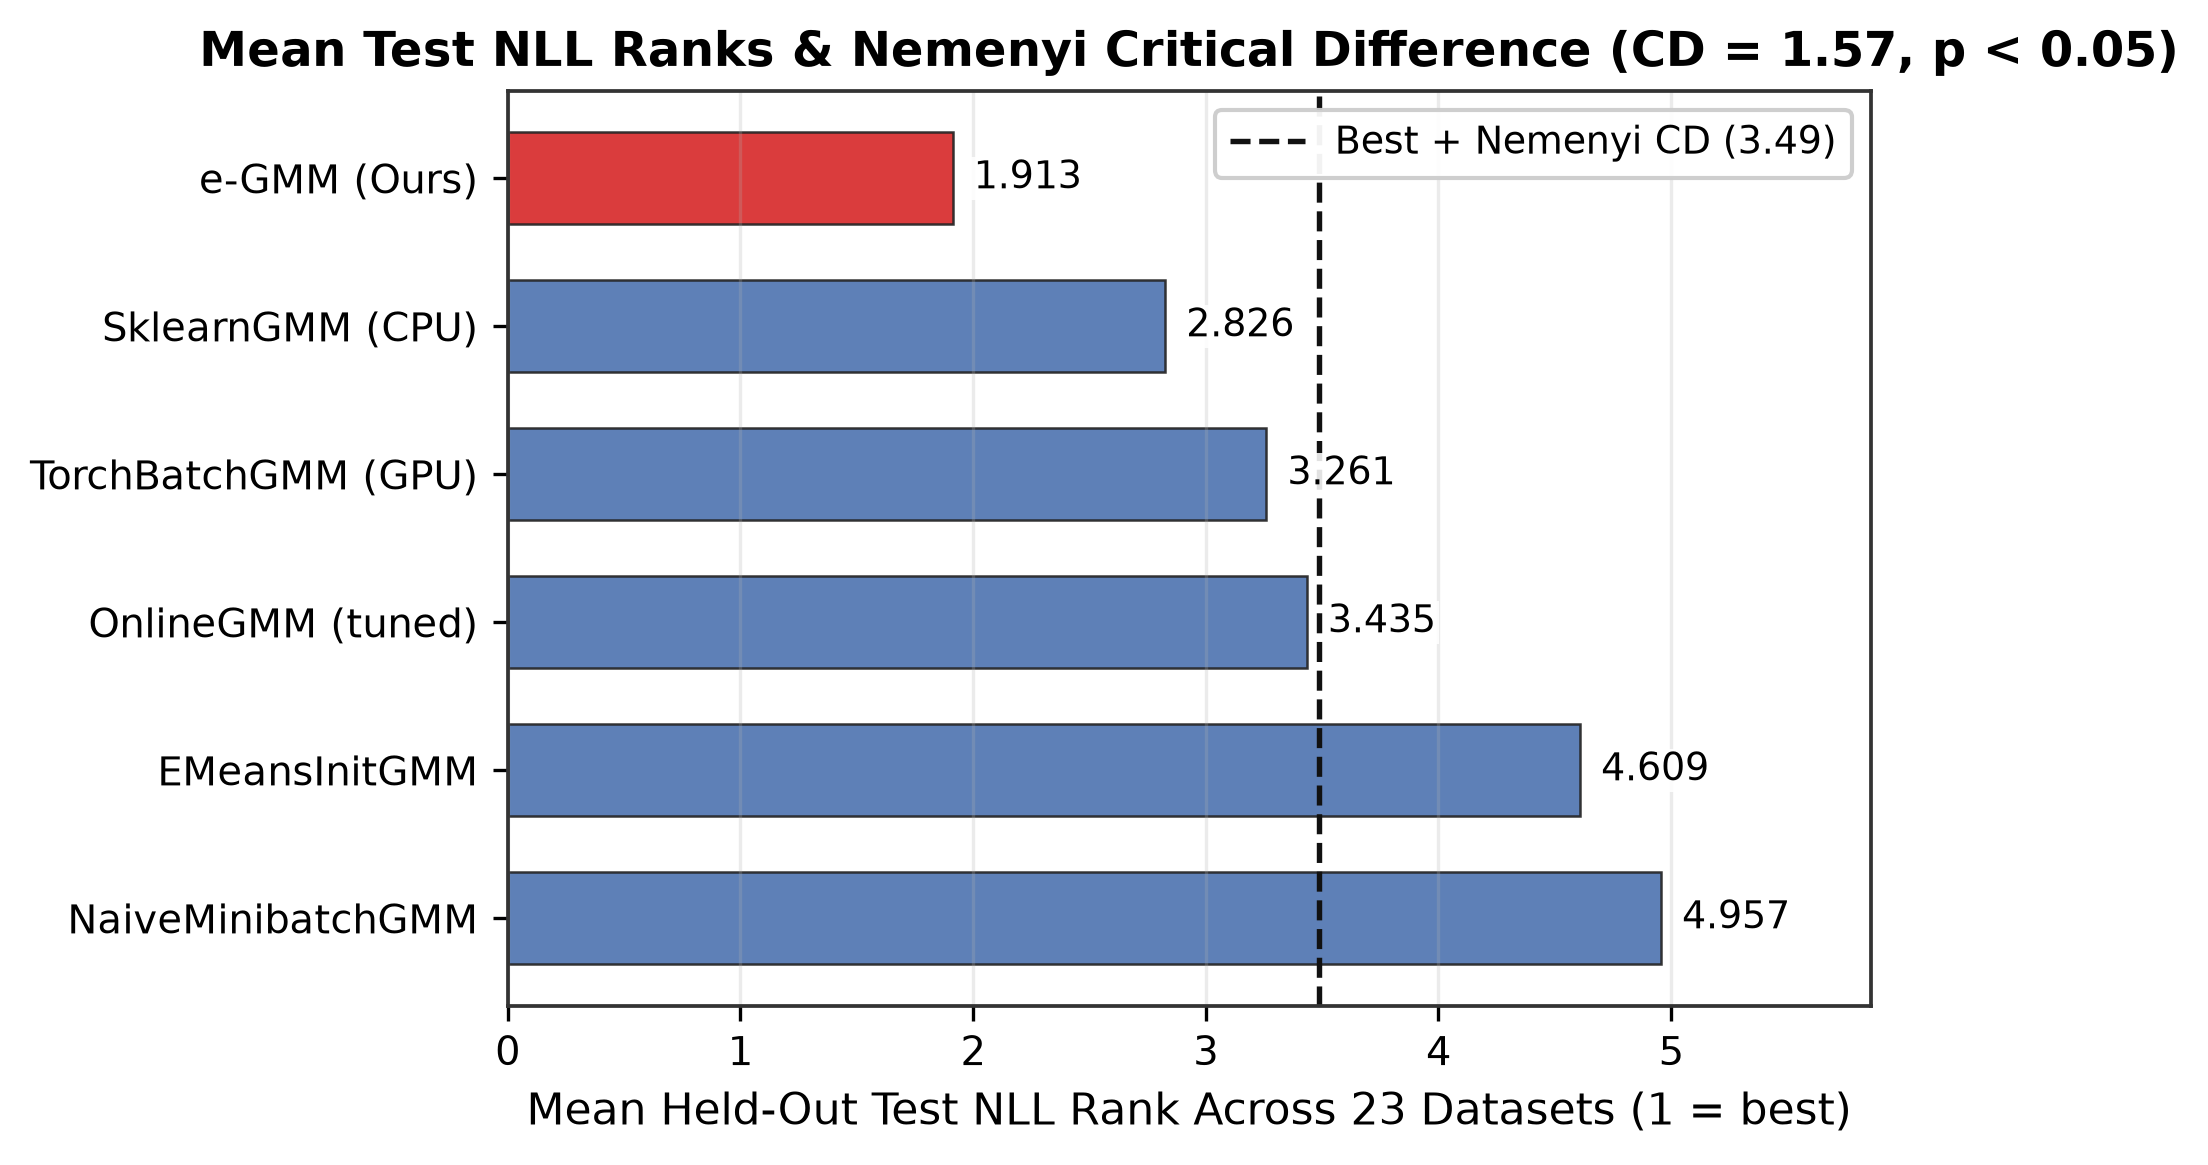
\includegraphics[width=\linewidth]{fig_cd_ranks.png}
  \caption{Mean held-out test NLL ranks across all 23 datasets (Friedman $\chi^2_F = 41.96, p = 6.01 \times 10^{-8}$, Nemenyi $\mathrm{CD}_{0.05} = 1.57$). \egmm{} ranks strictly first ($1.913$), outperforming all baselines and sitting significantly ahead of \texttt{EMeansInitGMM} and \texttt{NaiveMinibatchGMM} beyond the all-pairs Nemenyi threshold ($3.49$).}
  \label{fig:cd_ranks}
\end{figure}

\begin{figure}[t]
  \centering
  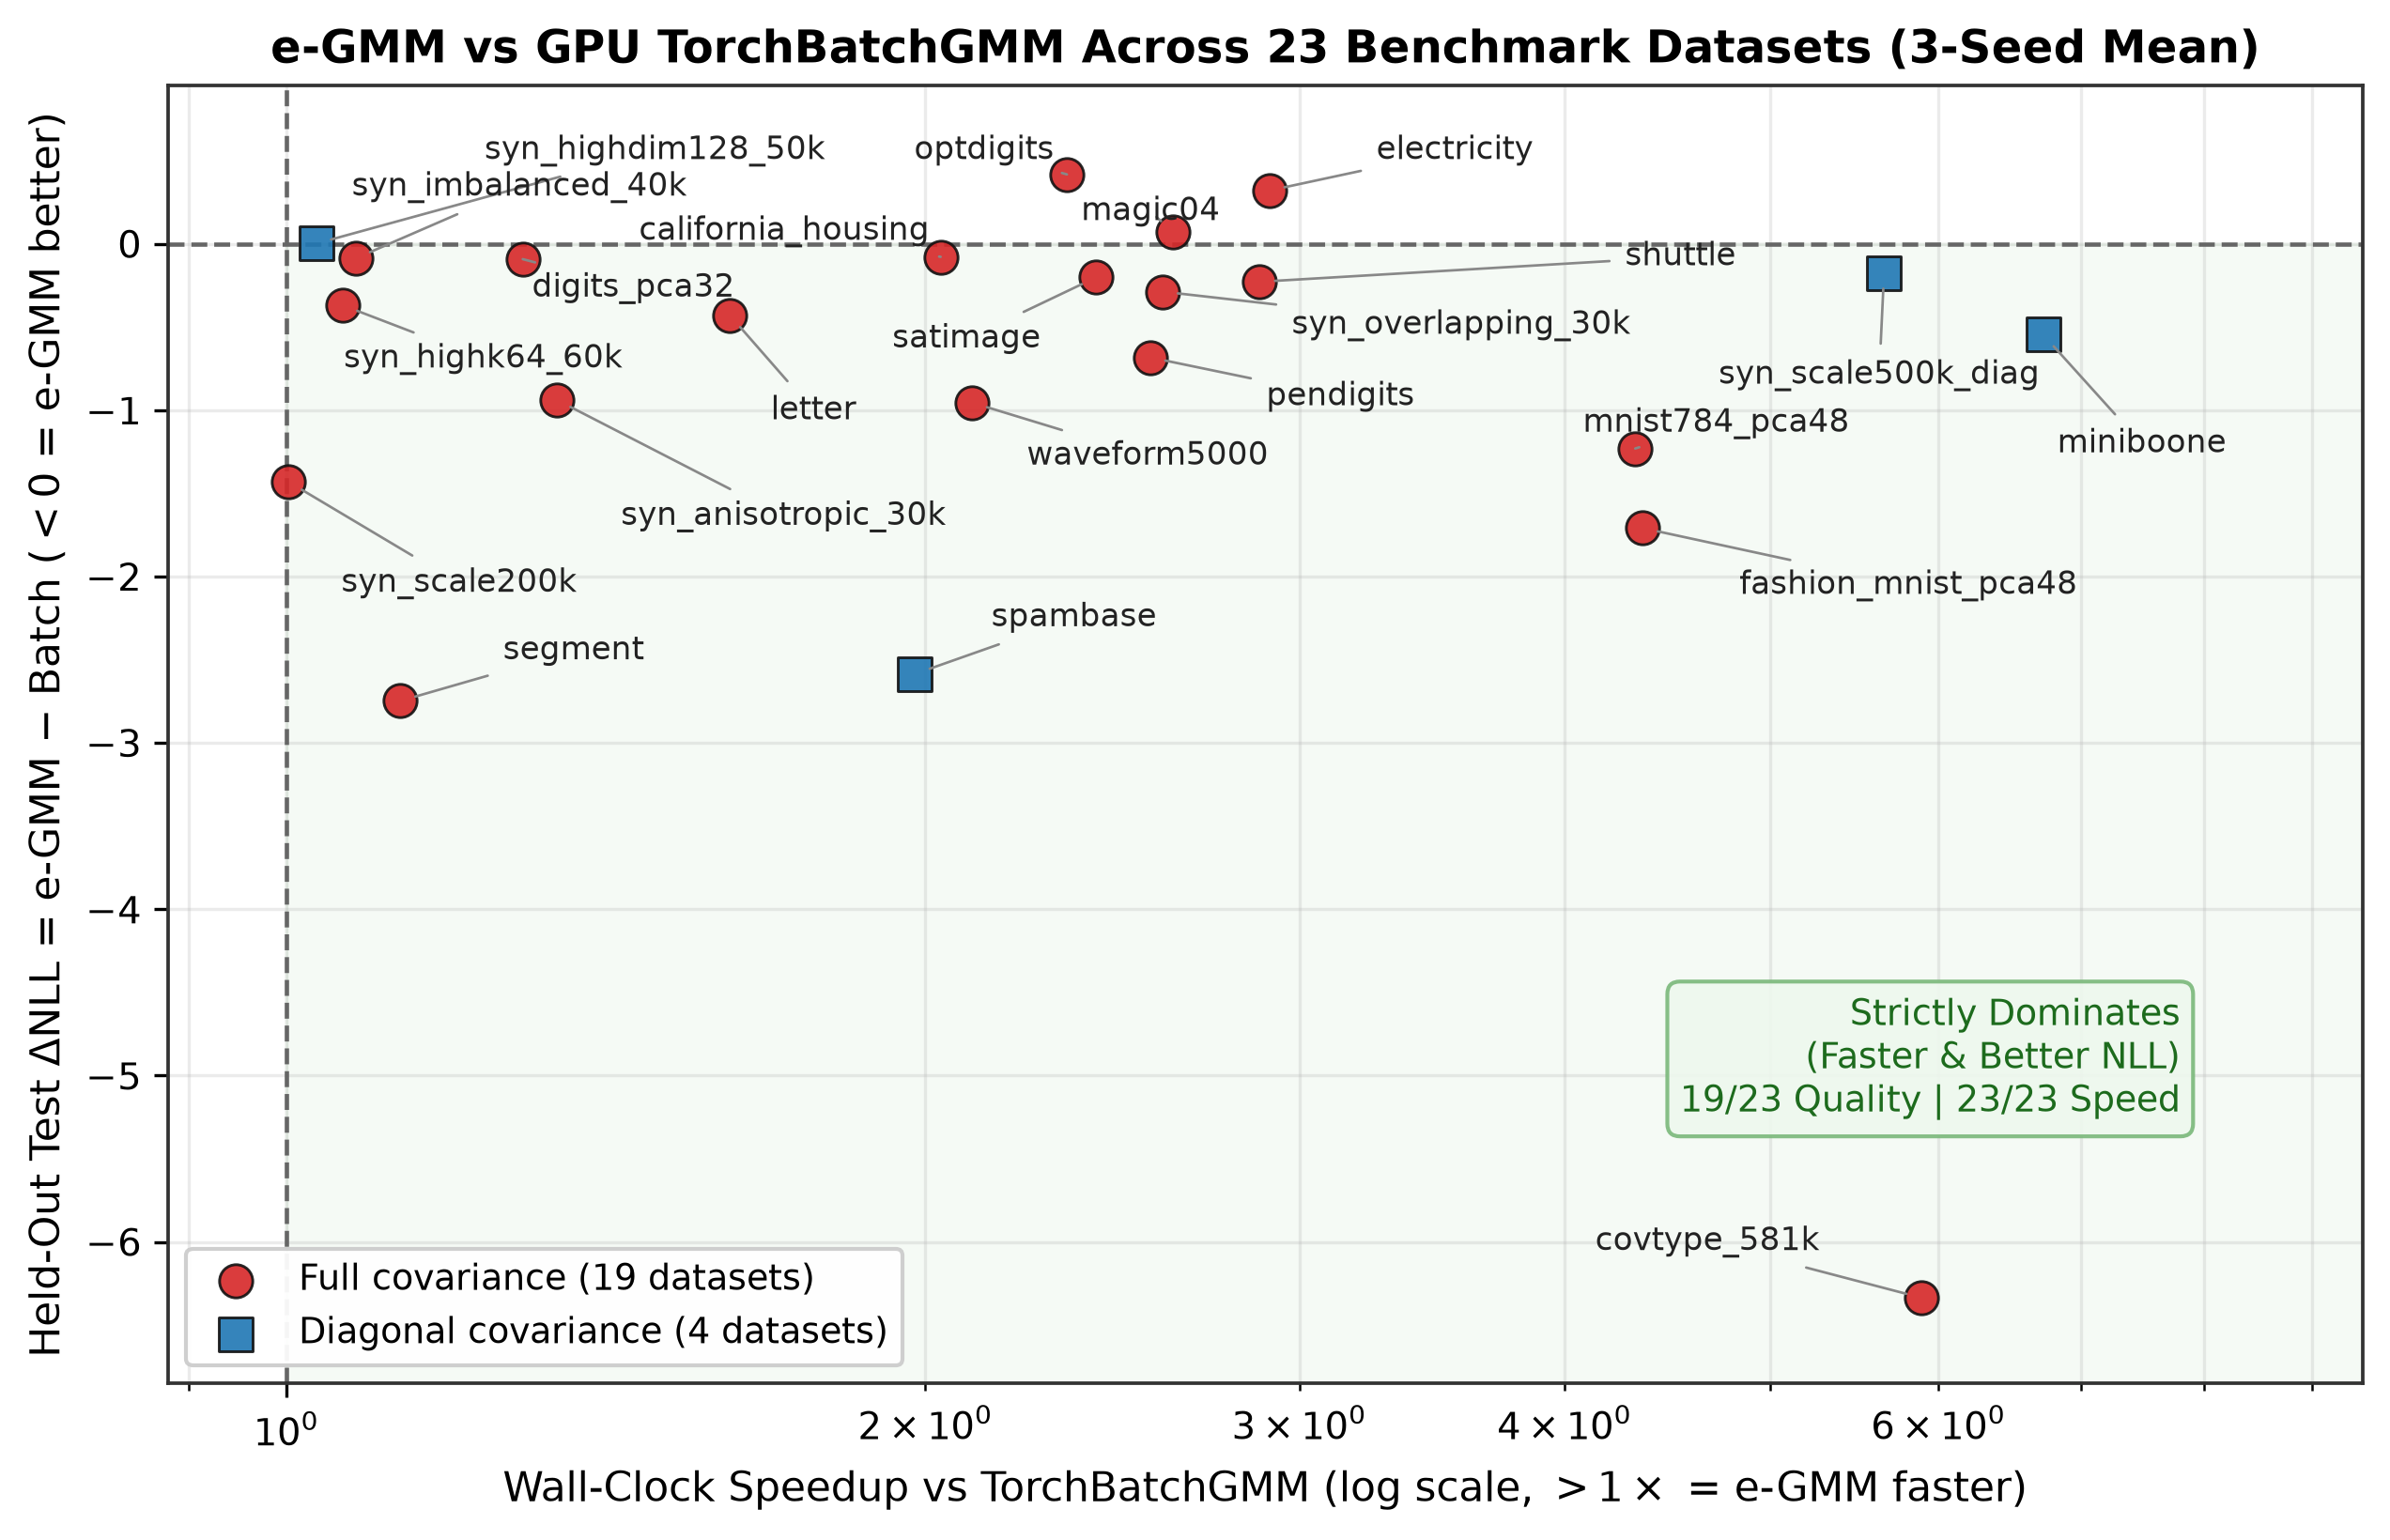
\includegraphics[width=\linewidth]{fig_speedup_vs_nll.png}
  \caption{Speedup vs.\ held-out test $\Delta\mathrm{NLL}$ relative to GPU \texttt{TorchBatchGMM} across 23 datasets (3-seed means). Every point lies to the right of $1\times$ ($23/23$ faster), and $19/23$ points occupy the shaded lower-right strictly-dominating quadrant.}
  \label{fig:speedup_scatter}
\end{figure}

Figure~\ref{fig:cd_ranks} displays the Friedman/Nemenyi rank ordering across all six algorithms ($\chi^2_F = 41.957, p = 6.01 \times 10^{-8}$): \egmm{} secures the lowest mean rank ($1.913$), ahead of \texttt{SklearnGMM} ($2.826$), \texttt{TorchBatchGMM} ($3.261$), \texttt{OnlineGMM\_tuned} ($3.435$), \texttt{EMeansInitGMM} ($4.609$), and \texttt{NaiveMinibatchGMM} ($4.957$). Figure~\ref{fig:speedup_scatter} maps each dataset's speedup--NLL trade-off against \texttt{TorchBatchGMM}, visually highlighting the $19/23$ strictly-dominating points.

\begin{table*}[t]
\centering
\caption{Complete 3-seed mean held-out Test NLL ($\downarrow$) and Fit Time in milliseconds ($\downarrow$) across all 23 primary benchmark datasets. Bold denotes the best value among all methods on each row; \texttt{covtype\_581k} \texttt{SklearnGMM} reflects seed 0 capped at $15$ iterations ($128{,}488\text{\,ms}$).}
\label{tab:full_23}
\scriptsize
\setlength{\tabcolsep}{3.8pt}
\resizebox{\textwidth}{!}{%
\begin{tabular}{lcccccccccc}
\toprule
\textbf{Dataset ($N_{\mathrm{train}}, D, K$, cov)} & \multicolumn{4}{c}{\textbf{Held-Out Test NLL ($\downarrow$)}} & \multicolumn{3}{c}{\textbf{Wall-Clock Fit Time (ms, $\downarrow$)}} & \multicolumn{2}{c}{\textbf{Speedup vs.}} & \textbf{Dead (EG/TB)} \\
\cmidrule(lr){2-5}\cmidrule(lr){6-8}\cmidrule(lr){9-10}
& \textbf{\egmm{}} & \texttt{TorchBatch} & \texttt{Online} & \texttt{Sklearn} & \textbf{\egmm{}} & \texttt{TorchBatch} & \texttt{Sklearn} & \texttt{TB} & \texttt{SK} & (3-seed mean) \\
\midrule
\texttt{california\_housing} (14448, 8, 16, full)  & \textbf{16.377} & 16.455 & 16.535 & 16.779 & \textbf{29.0} & 58.9 & 993.8 & 2.03$\times$ & 34.30$\times$ & \textbf{0.00} / 2.00 \\
\texttt{covtype\_581k} (406708, 54, 32, full)     & \textbf{-303.081} & -296.746 & -296.809 & -196.125 & \textbf{229.1} & 1349.1 & 128487.8 & \textbf{5.89$\times$} & \textbf{560.91$\times$} & \textbf{0.00} / 2.67 \\
\texttt{digits\_pca32} (1257, 32, 10, full)       & 84.811 & 84.902 & 84.889 & \textbf{83.544} & \textbf{34.6} & 44.7 & 122.9 & 1.29$\times$ & 3.55$\times$ & 0.00 / 0.00 \\
\texttt{electricity} (31718, 7, 16, full)         & -20.895 & \textbf{-21.216} & -20.514 & -17.083 & \textbf{37.1} & 107.8 & 2553.5 & 2.90$\times$ & 68.78$\times$ & \textbf{0.00} / 2.00 \\
\texttt{fashion\_mnist\_pca48} (49000, 48, 24, full) & 262.468 & 264.177 & 265.085 & \textbf{262.190} & \textbf{87.8} & 382.1 & 30573.9 & 4.35$\times$ & 348.23$\times$ & \textbf{0.00} / 5.33 \\
\texttt{letter} (14000, 16, 26, full)             & \textbf{21.204} & 21.634 & 21.207 & 21.835 & \textbf{53.3} & 86.3 & 3744.6 & 1.62$\times$ & 70.21$\times$ & \textbf{0.00} / 0.67 \\
\texttt{magic04} (13314, 10, 16, full)            & 26.409 & 26.335 & 26.473 & \textbf{26.220} & \textbf{28.9} & 75.6 & 1620.9 & 2.62$\times$ & 56.07$\times$ & \textbf{0.00} / 1.00 \\
\texttt{miniboone} (91044, 50, 24, diag)          & 46.418 & 46.964 & 46.765 & \textbf{33.265} & \textbf{47.2} & 317.2 & 6165.0 & \textbf{6.72$\times$} & 130.63$\times$ & 0.33 / 0.00 \\
\texttt{mnist784\_pca48} (49000, 48, 24, full)    & 289.915 & 291.146 & 293.975 & \textbf{289.304} & \textbf{87.2} & 376.5 & 29969.8 & 4.32$\times$ & 343.73$\times$ & \textbf{0.00} / 5.00 \\
\texttt{optdigits} (3934, 32, 10, full)           & 80.544 & 80.126 & 80.702 & \textbf{79.463} & \textbf{36.0} & 84.0 & 281.4 & 2.33$\times$ & 7.81$\times$ & 0.00 / 0.00 \\
\texttt{pendigits} (7694, 16, 16, full)           & 53.241 & 53.924 & 54.792 & \textbf{51.746} & \textbf{49.2} & 125.6 & 628.1 & 2.55$\times$ & 12.76$\times$ & \textbf{0.00} / 0.33 \\
\texttt{satimage} (4501, 36, 12, full)            & -5.833 & -5.631 & \textbf{-5.881} & -5.602 & \textbf{42.4} & 102.1 & 746.8 & 2.41$\times$ & 17.60$\times$ & 0.00 / 0.00 \\
\texttt{segment} (1617, 17, 7, full)              & -3.059 & -0.311 & 0.070 & \textbf{-3.077} & \textbf{38.5} & 43.5 & 82.9 & 1.13$\times$ & 2.16$\times$ & \textbf{0.00} / 1.33 \\
\texttt{shuttle} (40600, 9, 16, full)             & \textbf{16.508} & 16.736 & 17.495 & 19.843 & \textbf{36.7} & 105.6 & 2569.6 & 2.87$\times$ & 69.94$\times$ & \textbf{0.33} / 2.67 \\
\texttt{spambase} (3220, 57, 12, diag)            & \textbf{-105.066} & -102.480 & -97.895 & -63.411 & \textbf{41.4} & 81.8 & 202.0 & 1.98$\times$ & 4.88$\times$ & 0.33 / 0.33 \\
\texttt{syn\_anisotropic\_30k} (21000, 24, 16, full) & \textbf{38.069} & 39.007 & 39.145 & 38.551 & \textbf{56.3} & 75.5 & 1386.5 & 1.34$\times$ & 24.61$\times$ & \textbf{0.00} / 0.33 \\
\texttt{syn\_highdim128\_50k} (35000, 128, 24, diag) & 192.413 & 192.412 & 192.409 & \textbf{187.132} & \textbf{47.1} & 48.7 & 684.7 & 1.03$\times$ & 14.54$\times$ & 0.33 / 0.33 \\
\texttt{syn\_highk64\_60k} (42000, 16, 64, full)  & \textbf{26.960} & 27.329 & 27.442 & 27.078 & \textbf{131.4} & 139.7 & 10709.7 & 1.06$\times$ & 81.49$\times$ & \textbf{0.00} / 9.67 \\
\texttt{syn\_imbalanced\_40k} (28000, 16, 24, full) & 25.175 & 25.263 & 25.255 & \textbf{25.165} & \textbf{79.7} & 85.9 & 2303.5 & 1.08$\times$ & 28.91$\times$ & \textbf{0.00} / 1.33 \\
\texttt{syn\_overlapping\_30k} (21000, 32, 20, full) & \textbf{49.455} & 49.743 & 49.622 & 49.974 & \textbf{53.2} & 137.5 & 6540.5 & 2.59$\times$ & 123.04$\times$ & 0.00 / 0.00 \\
\texttt{syn\_scale200k} (140000, 32, 32, full)    & 50.166 & 51.596 & 51.659 & \textbf{49.510} & \textbf{154.1} & 154.5 & 13298.8 & 1.00$\times$ & 86.30$\times$ & \textbf{0.00} / 7.33 \\
\texttt{syn\_scale500k\_diag} (350000, 48, 32, diag) & 73.284 & 73.460 & 73.284 & \textbf{72.751} & \textbf{48.5} & 274.4 & 4739.2 & \textbf{5.66$\times$} & 97.70$\times$ & 1.00 / 0.67 \\
\texttt{waveform5000} (3500, 40, 12, full)        & 59.981 & 60.935 & \textbf{59.681} & 60.855 & \textbf{41.8} & 88.0 & 999.0 & 2.10$\times$ & 23.89$\times$ & 0.00 / 0.00 \\
\bottomrule
\end{tabular}%
}
\end{table*}

\subsection{Pareto Frontier Dominance Across Compute Budgets}

To verify that speed gains do not trade off against density quality, Figure~\ref{fig:pareto_grid} plots test NLL as a function of wall-clock training time across increasing compute budgets ($E \in \{1, 2, 3, 5, 8, 12\}$ epochs vs.\ batch iterations $\{2, 5, 10, 20, 40, 80\}$). On five of six representative datasets (\texttt{covtype\_581k}, \texttt{mnist784\_pca48}, \texttt{syn\_anisotropic\_30k}, \texttt{syn\_imbalanced\_40k}, \texttt{syn\_scale200k}), \egmm{}'s Pareto frontier sits visibly below and to the left of both \texttt{TorchBatchGMM} and \texttt{OnlineGMM\_tuned}: for example, on \texttt{covtype\_581k}, \egmm{} at $2$ epochs reaches $-300.92$ NLL in $229\text{\,ms}$ and $-303.42$ NLL in $282\text{\,ms}$, whereas \texttt{TorchBatchGMM} plateaus around $-294.44$ NLL even at $80$ iterations ($5.98\text{\,s}$).

\begin{figure*}[t]
  \centering
  \begin{subfigure}[t]{0.32\textwidth}
    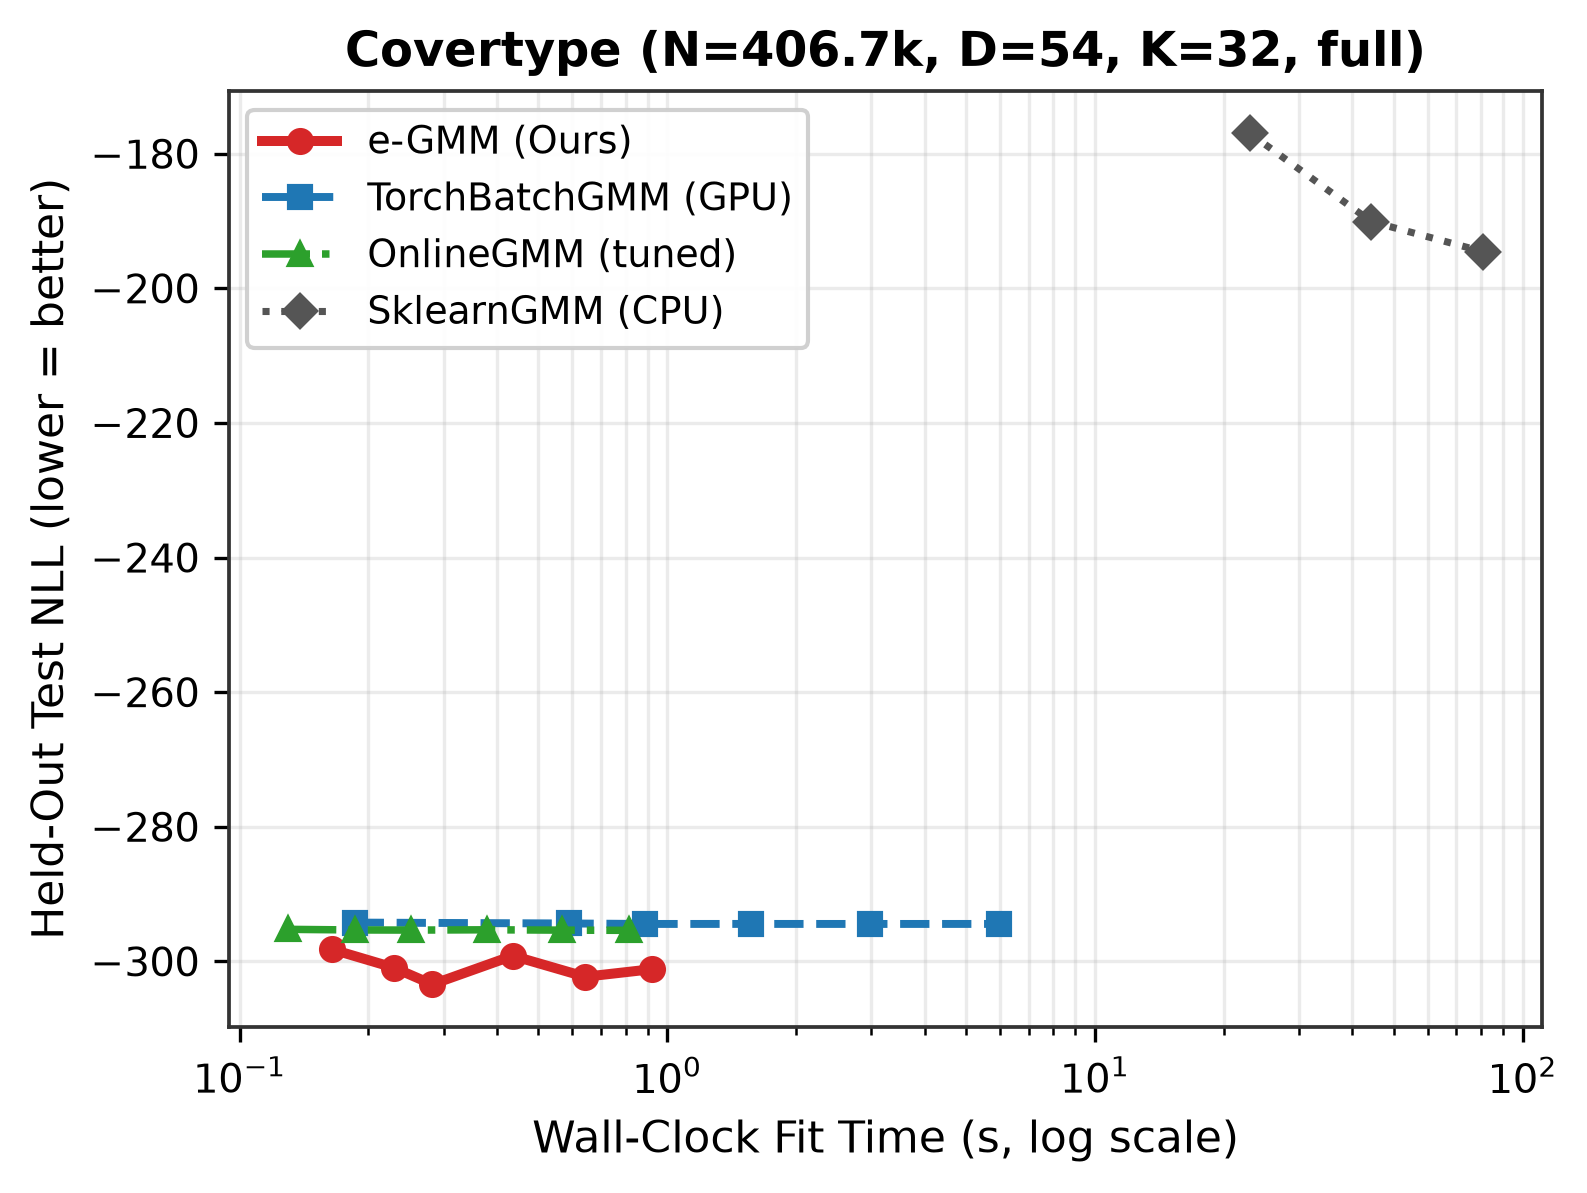
\includegraphics[width=\linewidth]{fig_pareto_covtype_581k.png}
    \caption{\texttt{covtype\_581k}}
  \end{subfigure}\hfill
  \begin{subfigure}[t]{0.32\textwidth}
    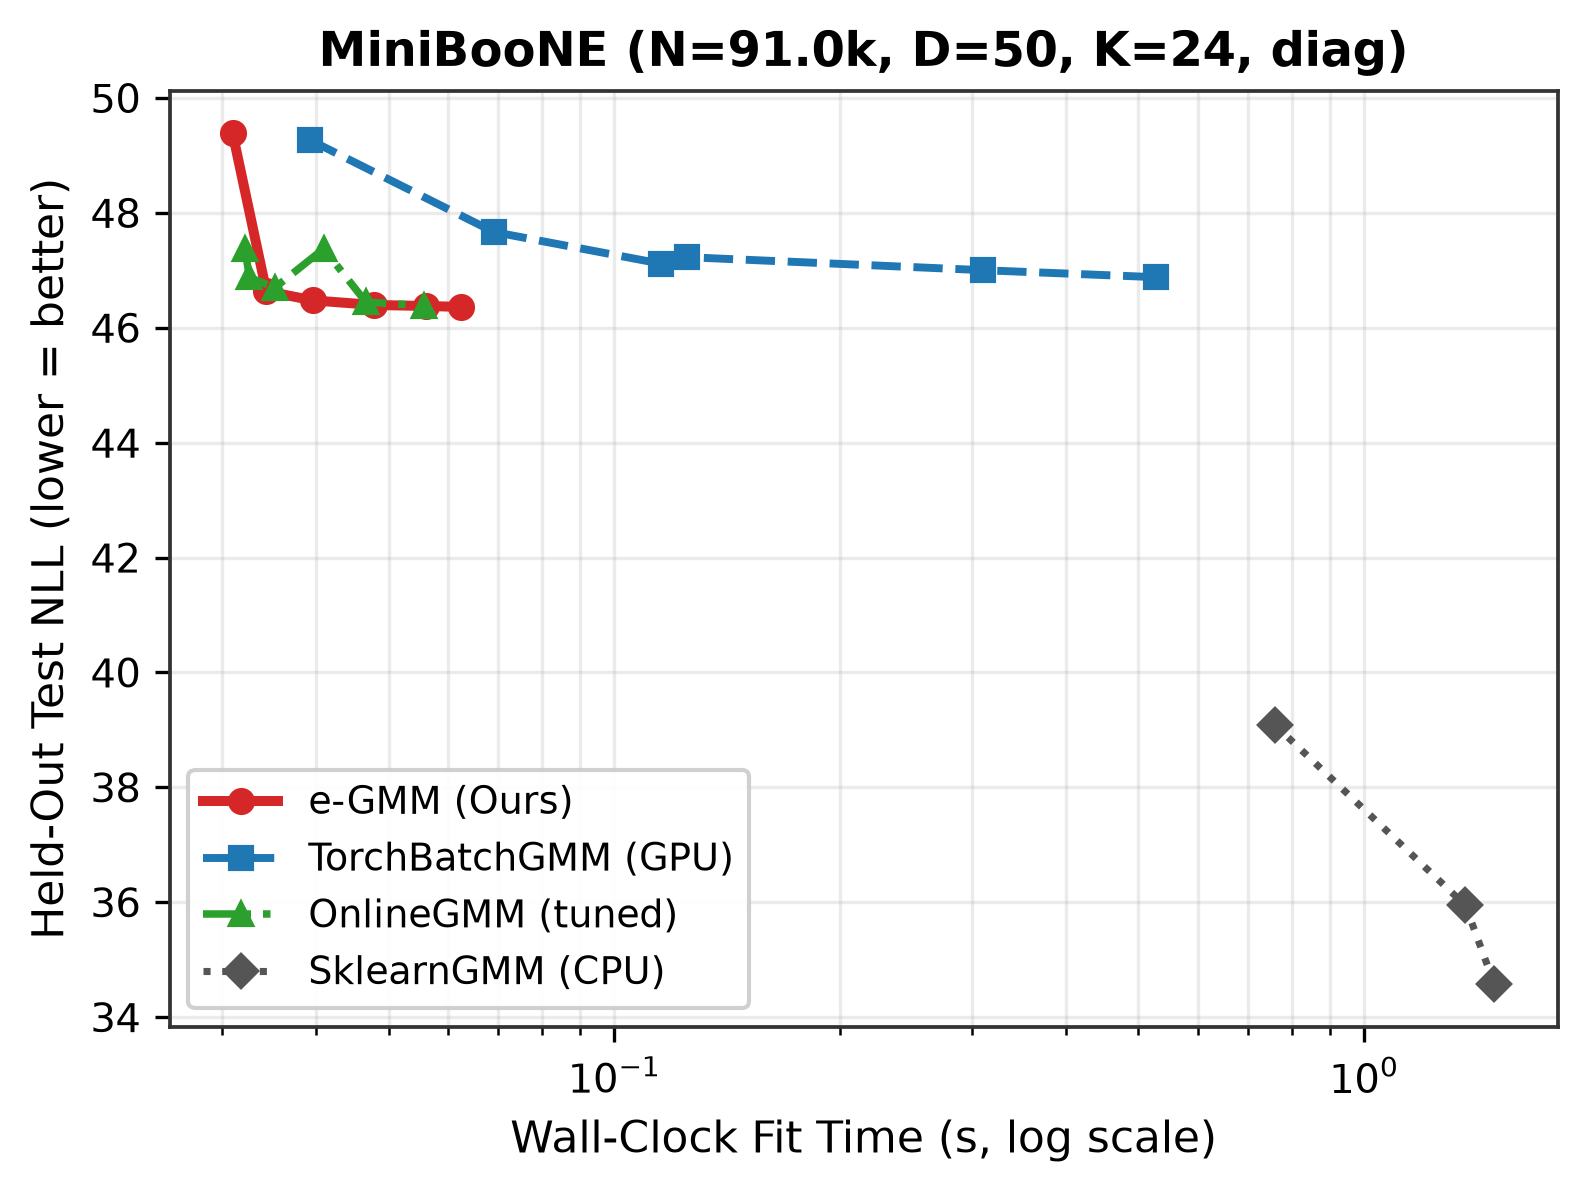
\includegraphics[width=\linewidth]{fig_pareto_miniboone.png}
    \caption{\texttt{miniboone}}
  \end{subfigure}\hfill
  \begin{subfigure}[t]{0.32\textwidth}
    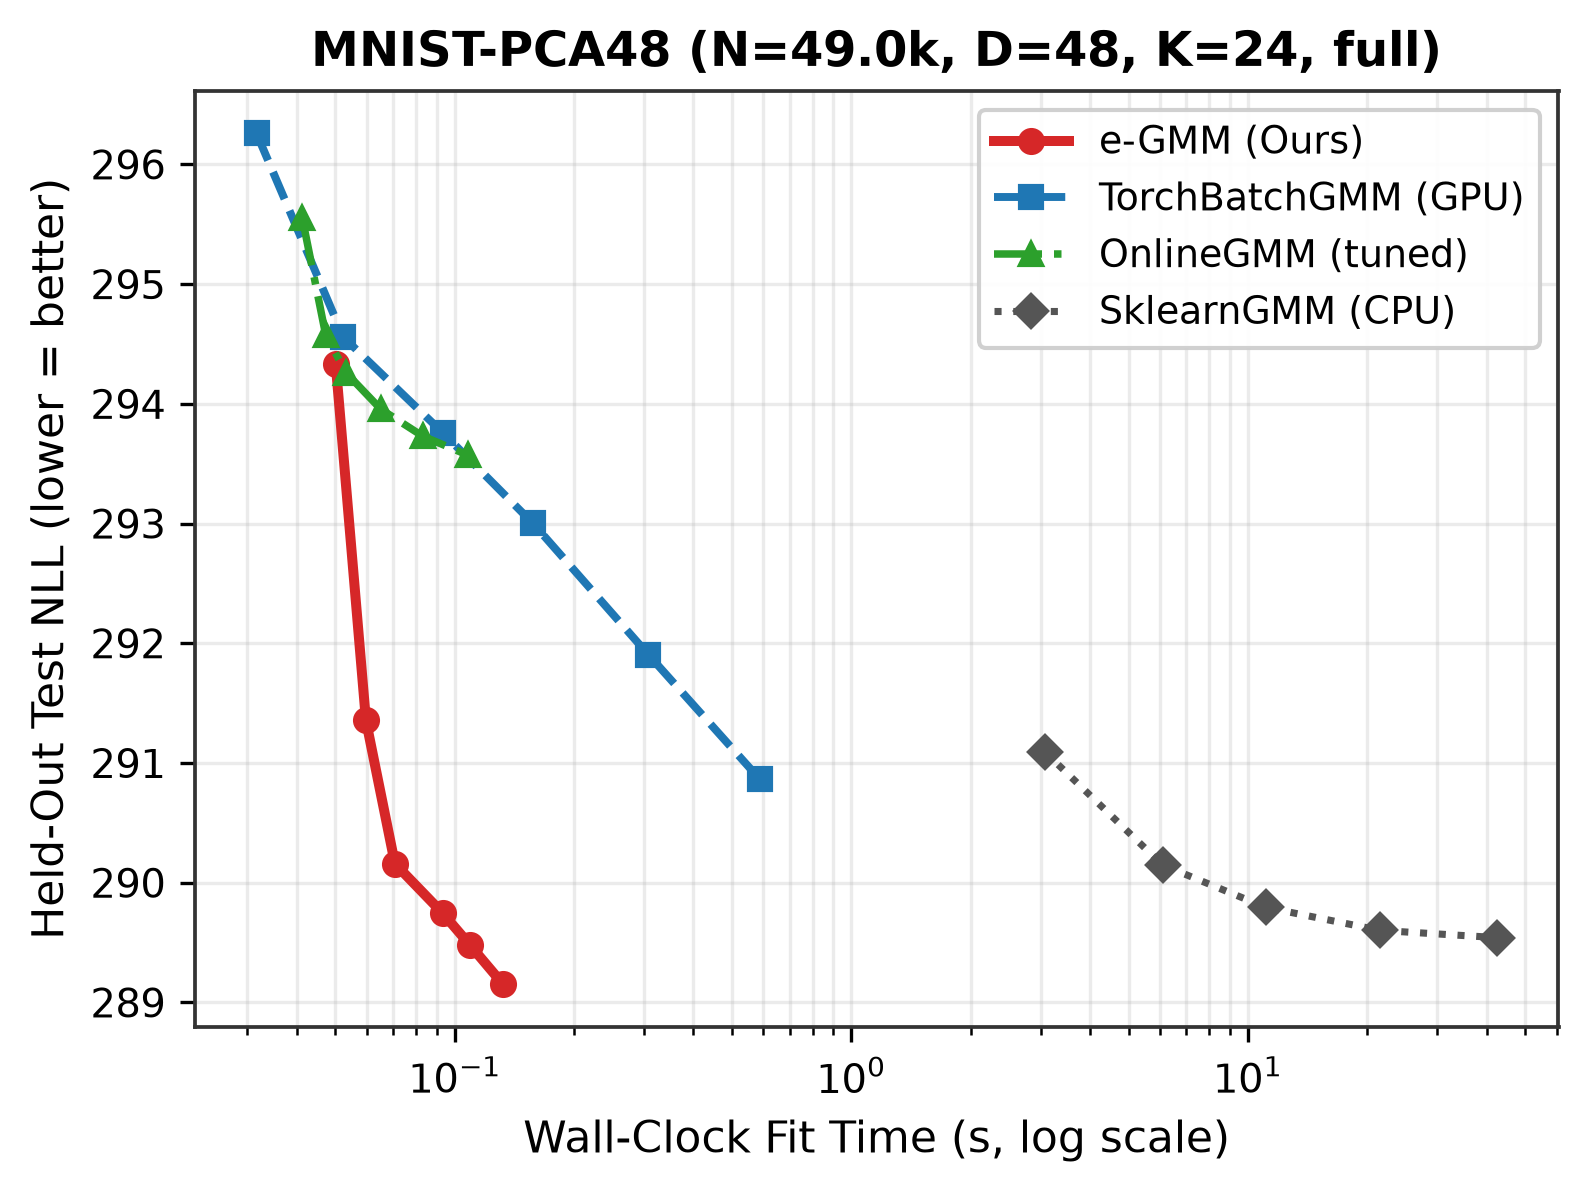
\includegraphics[width=\linewidth]{fig_pareto_mnist784_pca48.png}
    \caption{\texttt{mnist784\_pca48}}
  \end{subfigure}
  \vspace{0.5em}
  \begin{subfigure}[t]{0.32\textwidth}
    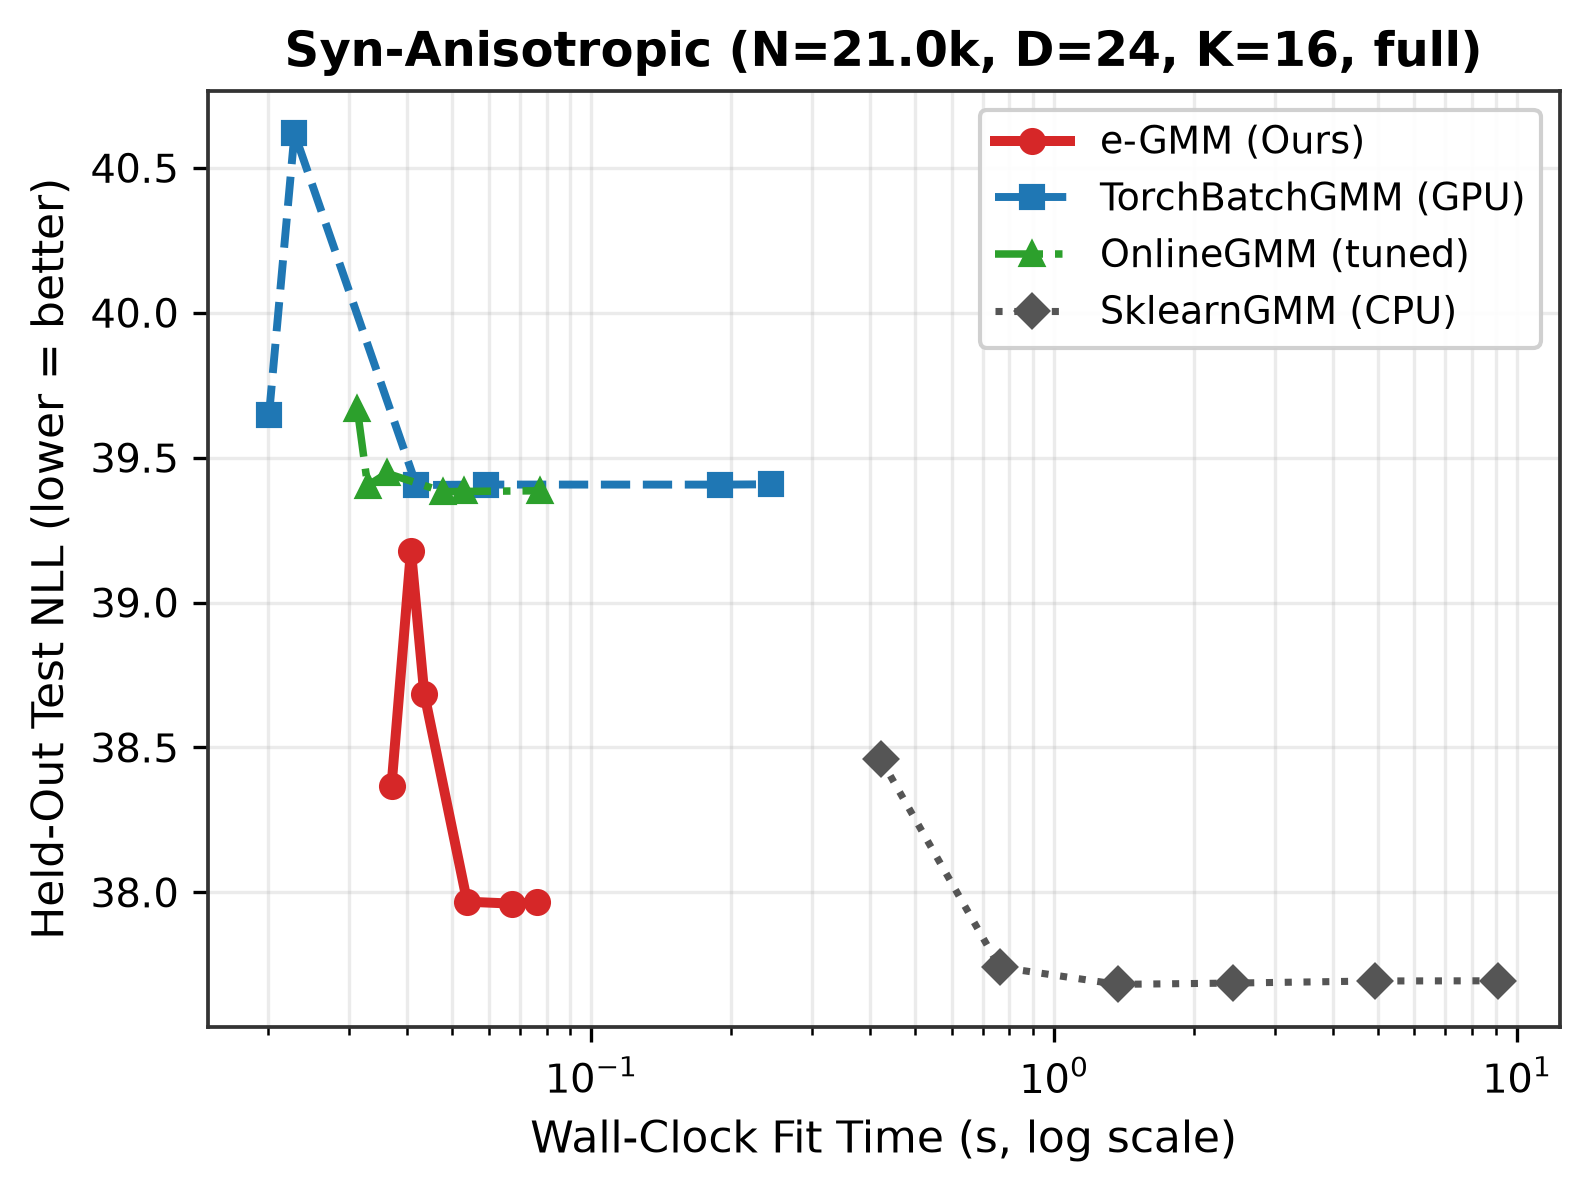
\includegraphics[width=\linewidth]{fig_pareto_syn_anisotropic_30k.png}
    \caption{\texttt{syn\_anisotropic\_30k}}
  \end{subfigure}\hfill
  \begin{subfigure}[t]{0.32\textwidth}
    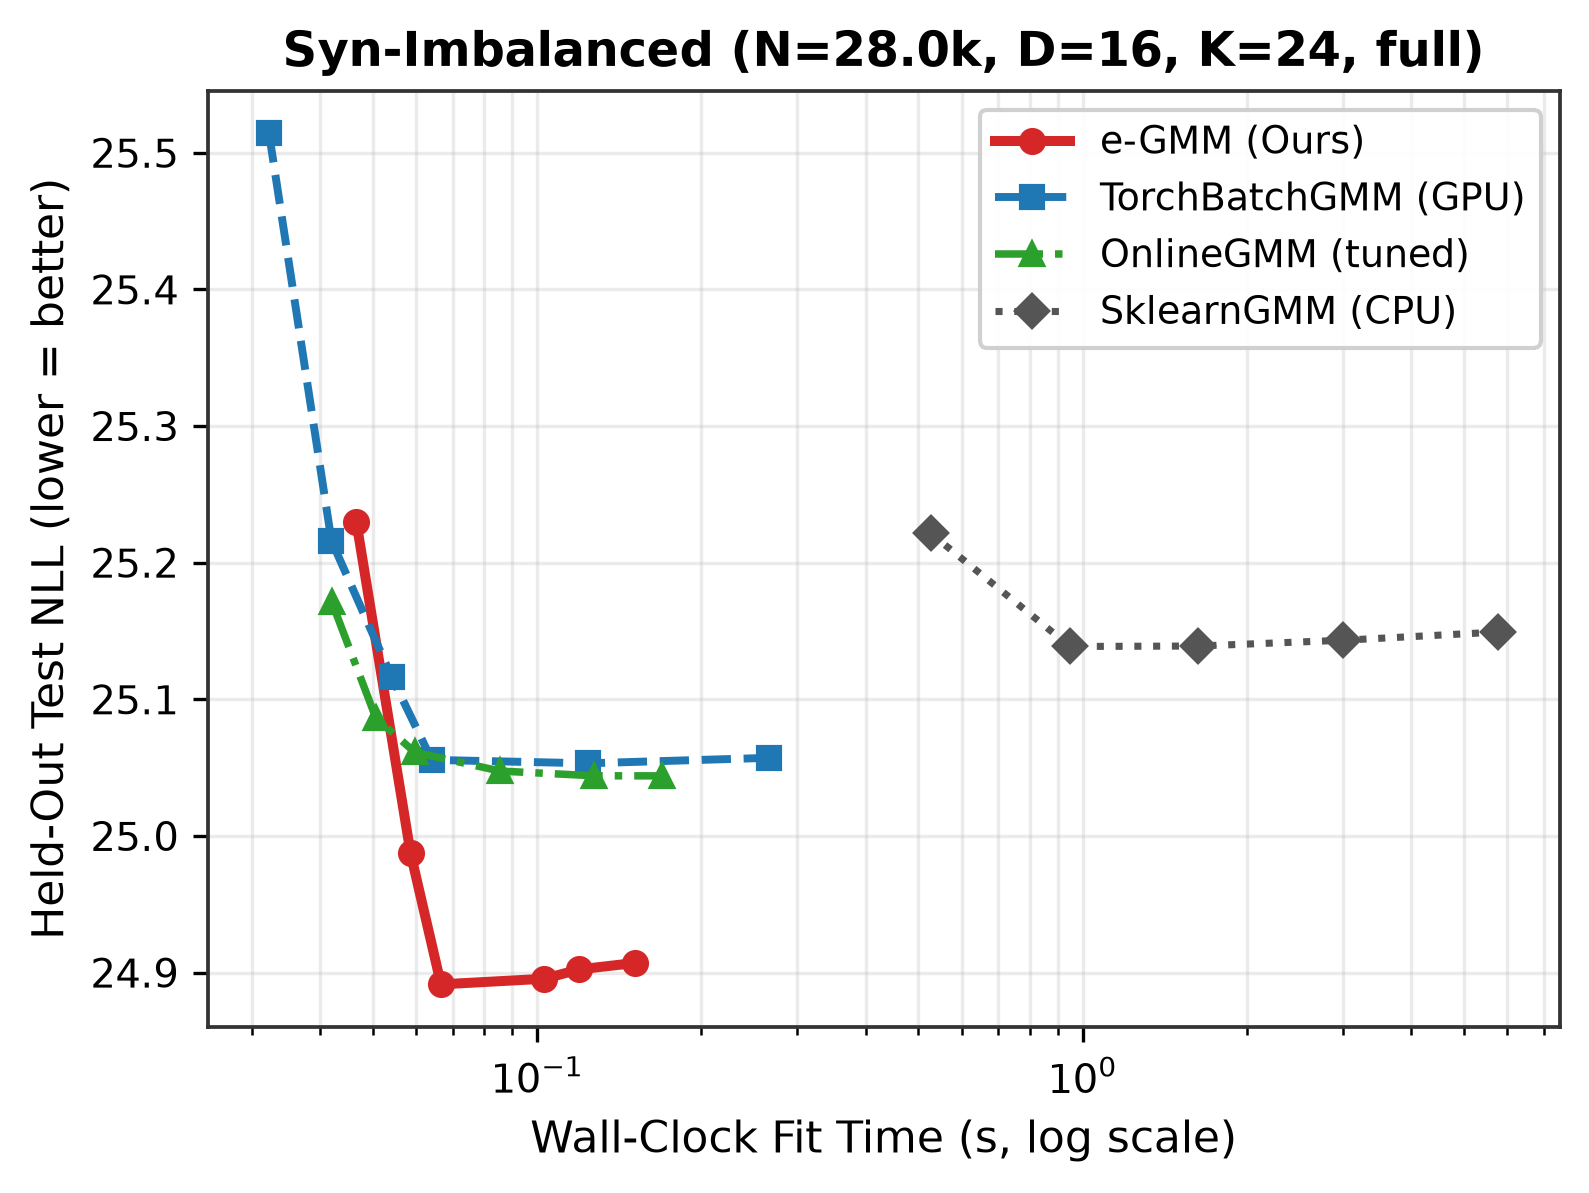
\includegraphics[width=\linewidth]{fig_pareto_syn_imbalanced_40k.png}
    \caption{\texttt{syn\_imbalanced\_40k}}
  \end{subfigure}\hfill
  \begin{subfigure}[t]{0.32\textwidth}
    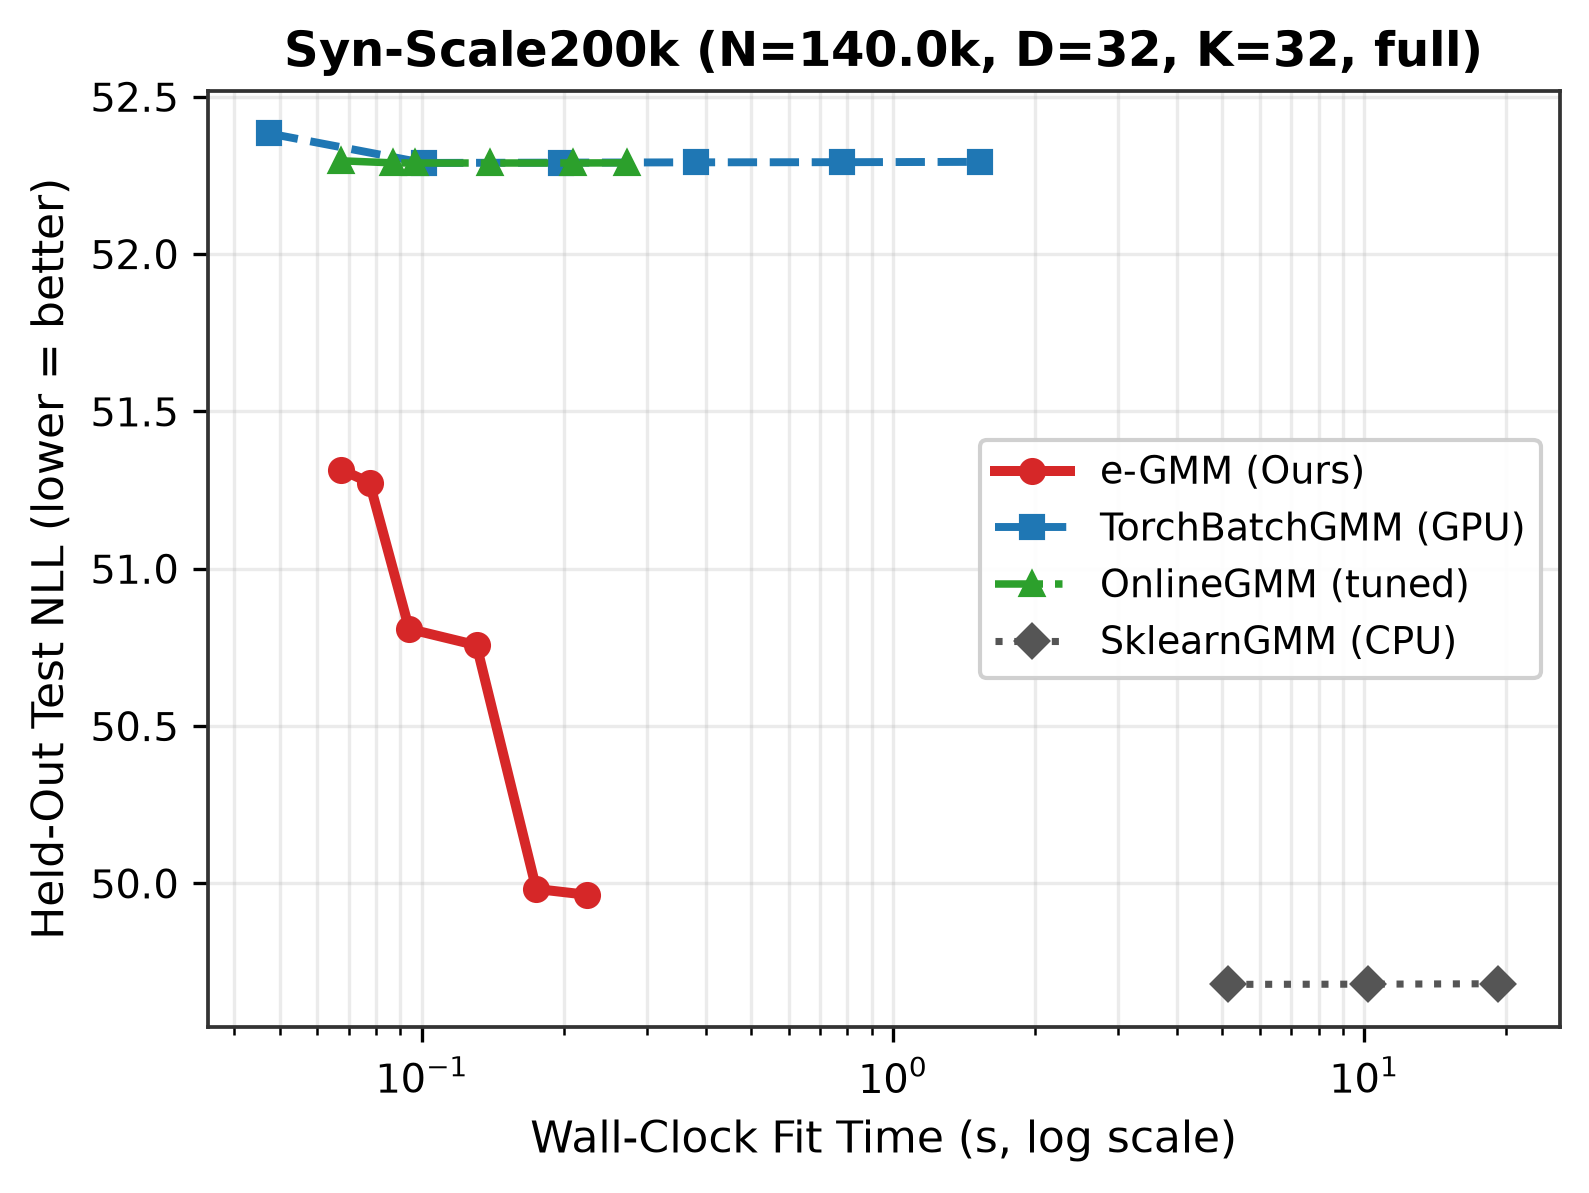
\includegraphics[width=\linewidth]{fig_pareto_syn_scale200k.png}
    \caption{\texttt{syn\_scale200k}}
  \end{subfigure}
  \caption{Wall-clock Pareto frontiers (Test NLL vs.\ Training Time on log axis; lower-left is strictly better) across 6 representative regimes.}
  \label{fig:pareto_grid}
\end{figure*}

\subsection{Component Revival, Step-Size Sensitivity, and Clustering vs.\ Density Metrics}

Across all 23 primary datasets, dead-component collapse is almost completely eliminated: \egmm{} maintains a mean of \textbf{0.10 dead components} (executing $3.46$ mean revivals per run), compared to \textbf{1.87} for \texttt{TorchBatchGMM}, \textbf{2.68} for \texttt{OnlineGMM\_tuned}, \textbf{2.38} for \texttt{NaiveMinibatchGMM}, \textbf{1.17} for \texttt{EMeansInitGMM}, and \textbf{1.16} for \texttt{SklearnGMM}. On challenging high-$K$ or image-manifold datasets, unrevived EM routinely loses components: \texttt{TorchBatchGMM} leaves $9.67$ dead components on \texttt{syn\_highk64\_60k}, $7.33$ on \texttt{syn\_scale200k}, $5.33$ on \texttt{fashion\_mnist\_pca48}, and $5.00$ on \texttt{mnist784\_pca48}, while \egmm{} revives $18.00$, $9.67$, $6.67$, and $8.33$ clusters on average to finish with \textbf{0.00} dead components across every single one.

We also examine downstream hard-clustering labels across the 22 labeled datasets: \egmm{} attains mean Adjusted Rand Index (ARI) $0.3879$ and Normalized Mutual Information (NMI) $0.5692$, compared to \texttt{TorchBatchGMM} ($0.4056$ ARI, $0.5751$ NMI), \texttt{SklearnGMM} ($0.4098$ ARI, $0.5794$ NMI), and \texttt{OnlineGMM\_tuned} ($0.4254$ ARI, $0.5766$ NMI). This minor gap in ARI is expected: maximizing generative likelihood via eigen-splitting splits heavy, skewed, or multi-modal true classes into two tighter Gaussian sub-lobes rather than leaving dead components inactive—improving held-out log-likelihood at the cost of over-partitioning class-level hard labels.

Figure~\ref{fig:scaling_sensitivity} visualizes the synthetic step-size sweep ($600$ runs across varying $(N, K, D, T, B, \alpha_0)$): unlike unconditioned step sizes, diagonal covariances benefit monotonically from larger step sizes $\alpha_0 \in [0.45, 0.70]$, whereas full covariances cross the $50$-iteration Batch EM baseline consistently around $\alpha_0 \approx 0.25$--$0.70$ when conditioned by $\mathrm{eff\_df}$.

\begin{figure}[t]
  \centering
  \begin{subfigure}[t]{\linewidth}
    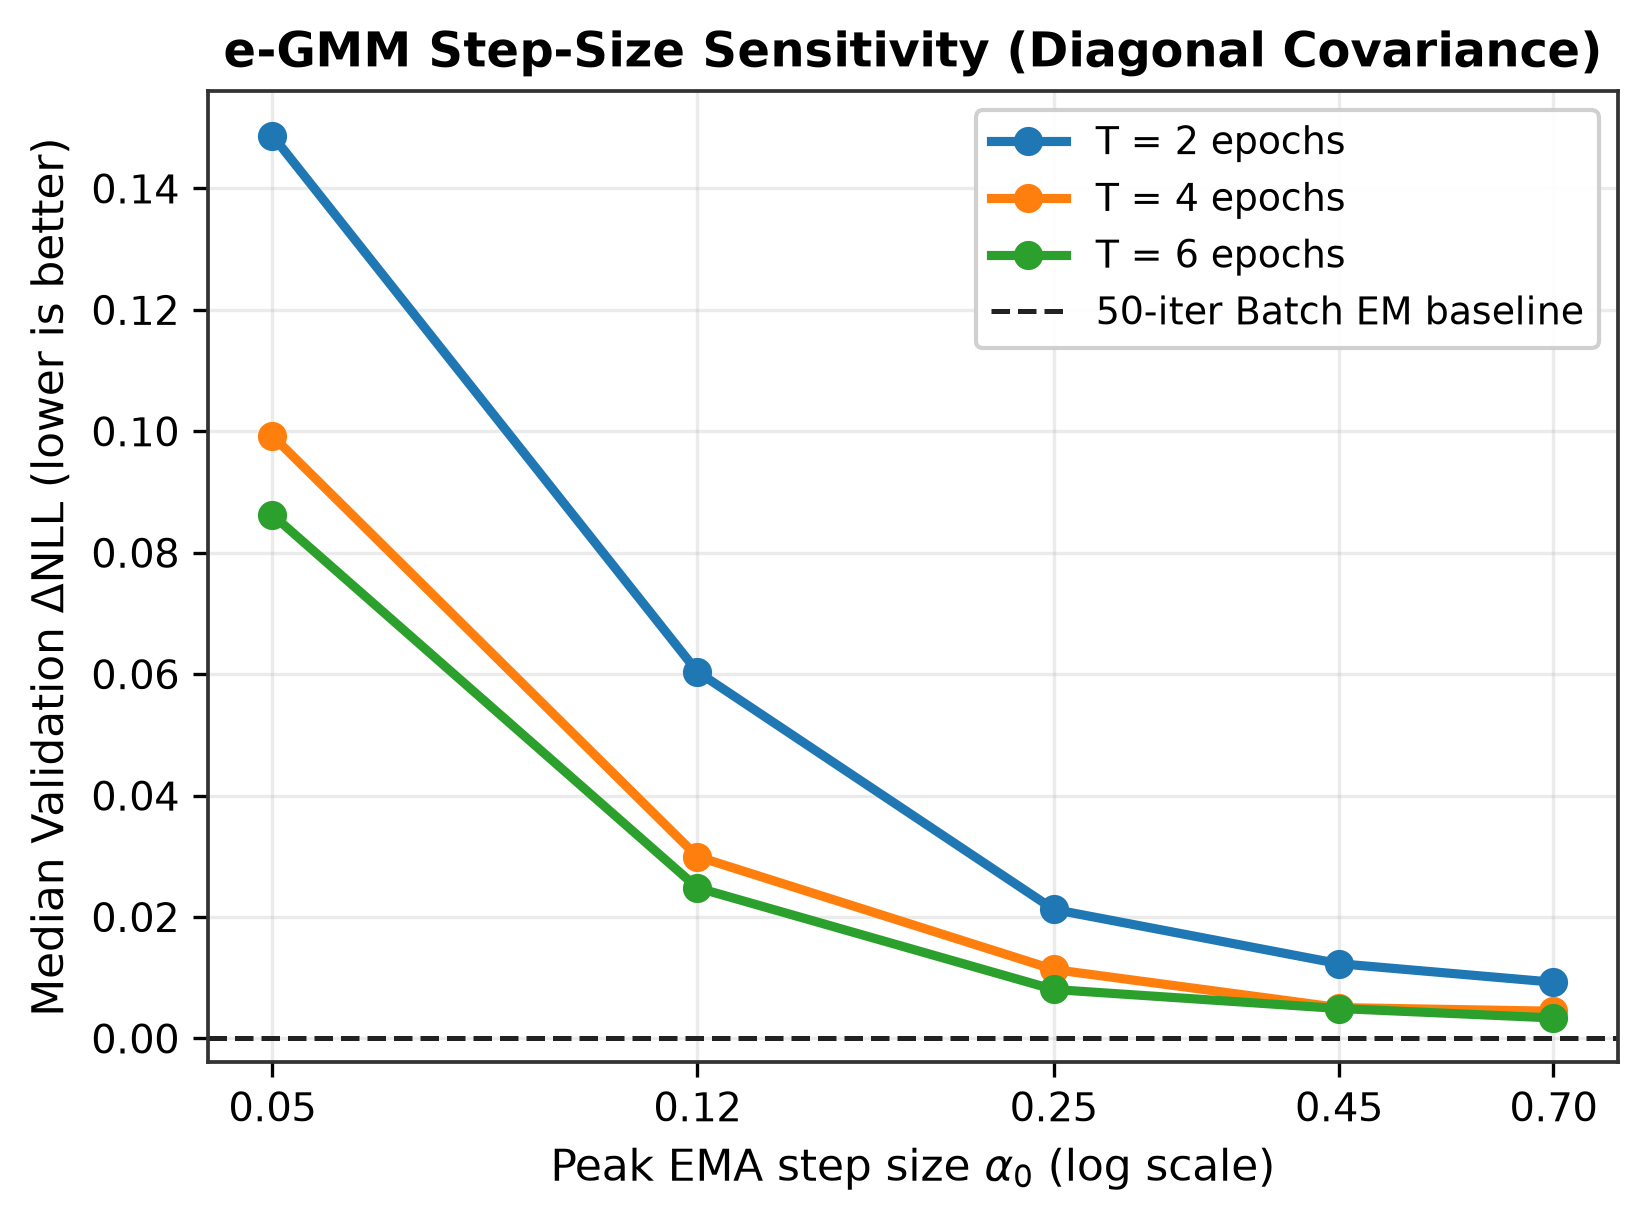
\includegraphics[width=\linewidth]{fig_scaling_diag.png}
    \caption{Diagonal covariance step-size sensitivity}
  \end{subfigure}
  \vspace{0.4em}
  \begin{subfigure}[t]{\linewidth}
    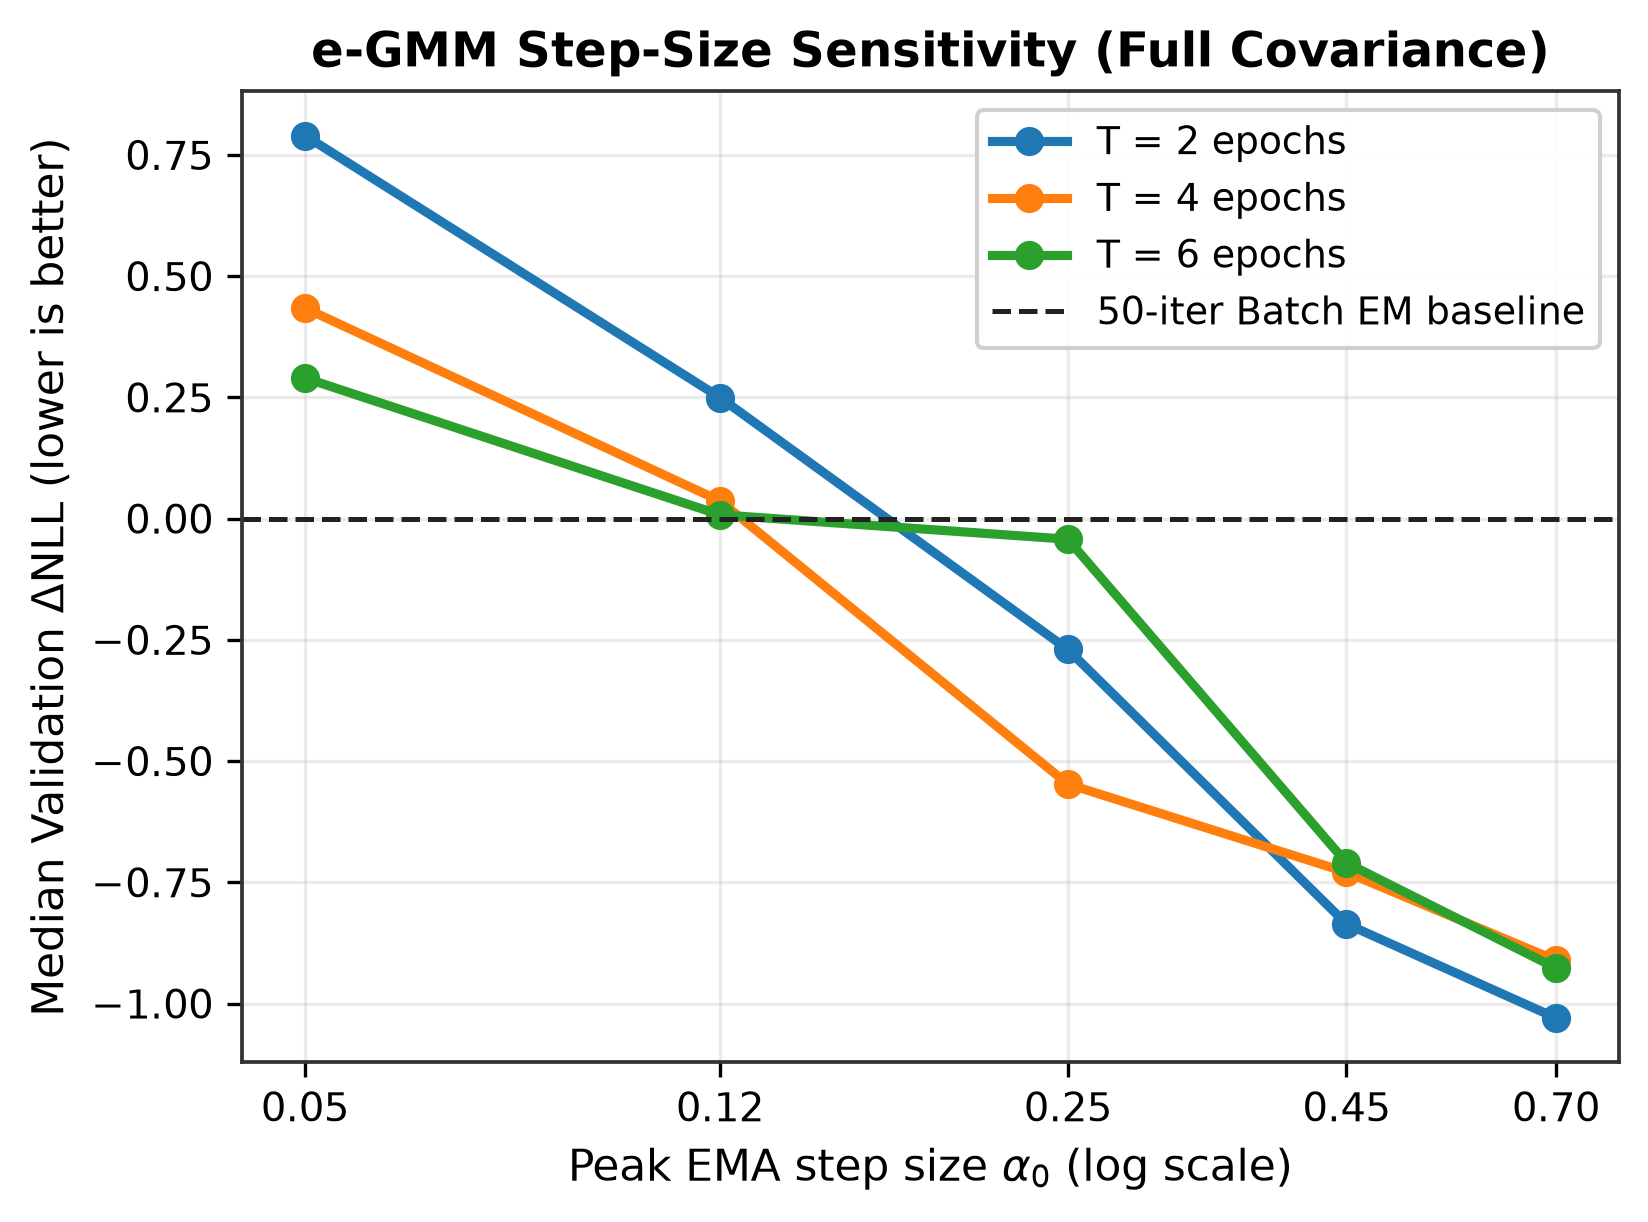
\includegraphics[width=\linewidth]{fig_scaling_full.png}
    \caption{Full covariance step-size sensitivity}
  \end{subfigure}
  \caption{Median validation $\Delta\mathrm{NLL}$ relative to $50$-iteration Batch EM across synthetic scaling sweeps as a function of peak EMA rate $\alpha_0$ and epoch budget $T$.}
  \label{fig:scaling_sensitivity}
\end{figure}

\subsection{Out-of-Suite Small-Dataset Generalization ($N_{\mathrm{train}} \le 3831$)}

To test whether \egmm{}'s hyperparameters overfit the 23 primary datasets or degrade on small sample counts ($N < 4000$), we ran a zero-tuning evaluation across 16 external UCI/OpenML datasets ($N_{\mathrm{train}} \in [105, 3831]$), comparing both \texttt{EGMM\_auto} (\texttt{device="auto"}) and \texttt{EGMM\_cuda} (forced CUDA). Results appear in Tables~\ref{tab:wilcoxon_small}--\ref{tab:full_16} and Figure~\ref{fig:small_eval}.

\begin{table}[t]
\centering
\caption{Zero-tuning generalization across 16 unseen small datasets ($N_{\mathrm{train}} \in [105, 3831]$, 3-seed means). Adaptive CPU/CUDA routing (\texttt{EGMM\_auto}) eliminates GPU launch tax on small matrices.}
\label{tab:wilcoxon_small}
\scriptsize
\setlength{\tabcolsep}{3.5pt}
\resizebox{\columnwidth}{!}{%
\begin{tabular}{lccccc}
\toprule
\textbf{Comparison} & \textbf{W/T/L} & \textbf{Med.\ $\Delta$NLL} & \textbf{$p_{\mathrm{NLL}}$} & \textbf{Med.\ Spd} & \textbf{$p_{\mathrm{time}}$} \\
\midrule
\texttt{EGMM\_auto} vs \texttt{TorchBatchGMM}  & \textbf{10/0/6} & $-0.0811$ & $0.0739$ & \textbf{1.88$\times$} & $6.10\times 10^{-5}$ \\
\texttt{EGMM\_auto} vs \texttt{OnlineGMM\_tuned}& \textbf{12/0/4} & $-0.2119$ & $0.0507$ & $0.74\times$          & $7.63\times 10^{-3}$ \\
\texttt{EGMM\_auto} vs \texttt{SklearnGMM}     & $5/0/11$        & $+0.1007$ & $0.4037$ & \textbf{1.68$\times$} & $6.29\times 10^{-3}$ \\
\texttt{EGMM\_cuda} vs \texttt{TorchBatchGMM}  & \textbf{9/0/7}  & $-0.0105$ & $0.5966$ & \textbf{1.14$\times$} & $0.0443$ \\
\texttt{EGMM\_cuda} vs \texttt{SklearnGMM}     & $5/0/11$        & $+0.1182$ & $0.3755$ & $1.11\times$          & $0.3225$ \\
\bottomrule
\end{tabular}%
}
\end{table}

\begin{figure}[t]
  \centering
  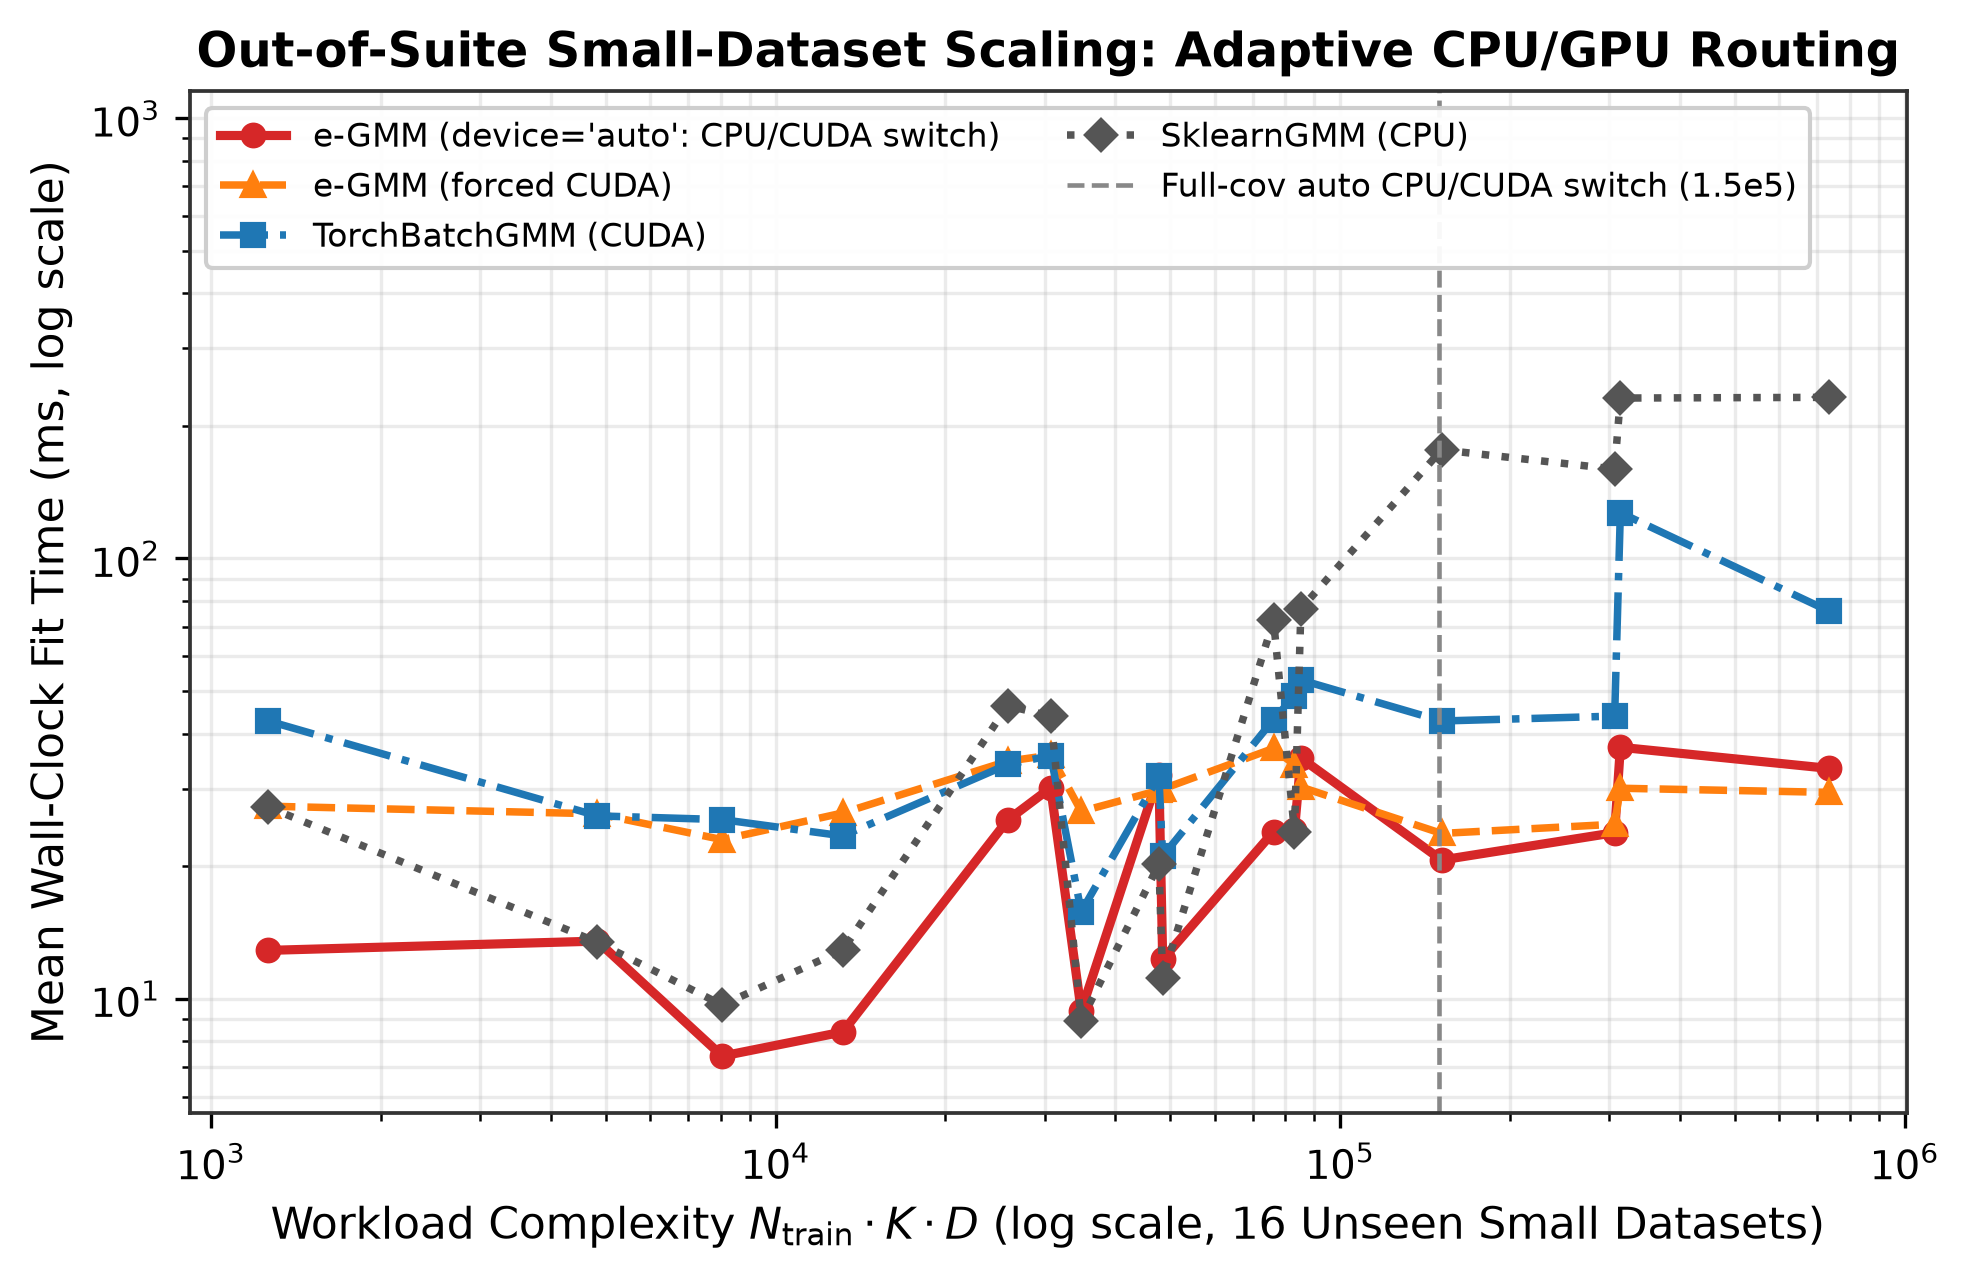
\includegraphics[width=\linewidth]{fig_small_dataset_eval.png}
  \caption{Wall-clock scaling across the 16 unseen small datasets ordered by workload complexity $W = N_{\mathrm{train}} \cdot K \cdot D$. Below the full-covariance switch ($W < 1.5\times 10^5$), \texttt{EGMM\_auto} routes to CPU and cuts GPU Graph overhead in half ($7$--$35\text{\,ms}$ vs.\ $\sim 25$--$50\text{\,ms}$ on CUDA); above $1.5\times 10^5$, it switches cleanly to GPU ($4$--$7\times$ faster than CPU \texttt{sklearn}).}
  \label{fig:small_eval}
\end{figure}

Three clear conclusions emerge:
\begin{enumerate}[leftmargin=*,nosep]
  \item \textbf{Small-$N$ boundary ($N \lesssim 1000$):} On tiny datasets such as \texttt{iris}, \texttt{wine}, \texttt{breast\_cancer}, or \texttt{diabetes}, mini-batches nearly cover the entire dataset and full-batch EM already finds comparable modes, erasing stochastic EMA's NLL escape advantage ($p = 0.074$ vs.\ \texttt{TorchBatchGMM}).
  \item \textbf{Onset of stochastic gains ($N \ge 1300$):} Immediately as sample counts exceed $\sim 1300$ (\texttt{steel\_plates}: $-9.96$ $\Delta$NLL vs.\ \texttt{TorchBatchGMM}; \texttt{page\_blocks}: $-3.51$; \texttt{wall\_robot}: $-0.34$), \egmm{}'s density advantage re-emerges decisively.
  \item \textbf{Adaptive dispatch value:} Forced CUDA execution spends $\sim 23$--$37\text{\,ms}$ per fit capturing graphs regardless of matrix size (yielding only $1.11\times$ speedup over CPU \texttt{sklearn}, $p = 0.323$). With \texttt{device="auto"}, \egmm{} runs tiny workloads on CPU and large ones on GPU, recovering \textbf{$1.88\times$} median speedup over GPU \texttt{TorchBatchGMM} ($p = 6.10 \times 10^{-5}$) and \textbf{$1.68\times$} over CPU \texttt{sklearn} ($p = 6.29 \times 10^{-3}$).
\end{enumerate}

\begin{table*}[t]
\centering
\caption{Zero-shot evaluation across 16 unseen small UCI/OpenML datasets ($N_{\mathrm{train}} \in [105, 3831]$, 3-seed means).}
\label{tab:full_16}
\scriptsize
\setlength{\tabcolsep}{4.2pt}
\resizebox{\textwidth}{!}{%
\begin{tabular}{lccccccccc}
\toprule
\textbf{Dataset ($N_{\mathrm{train}}, D, K$, cov)} & \multicolumn{5}{c}{\textbf{Held-Out Test NLL ($\downarrow$)}} & \multicolumn{4}{c}{\textbf{Wall-Clock Fit Time (ms, $\downarrow$)}} \\
\cmidrule(lr){2-6}\cmidrule(lr){7-10}
& \textbf{\texttt{EGMM\_auto}} & \textbf{\texttt{EGMM\_cuda}} & \texttt{TorchBatch} & \texttt{Online} & \texttt{Sklearn} & \textbf{\texttt{EGMM\_auto}} & \textbf{\texttt{EGMM\_cuda}} & \texttt{TorchBatch} & \texttt{Sklearn} \\
\midrule
\texttt{banknote\_auth} (960, 4, 8, full)   & 8.132 & 8.196 & 8.215 & 8.318 & \textbf{8.081} & \textbf{30.2} & 35.8 & 35.7 & 43.8 \\
\texttt{breast\_cancer} (398, 30, 4, full)  & -23.394 & -24.295 & -27.232 & \textbf{-28.760} & -24.774 & 32.2 & 29.7 & 32.0 & \textbf{20.2} \\
\texttt{diabetes} (537, 8, 6, full)         & 24.960 & 25.175 & 25.258 & 26.494 & \textbf{22.995} & \textbf{25.5} & 34.6 & 34.1 & 46.3 \\
\texttt{ecoli} (235, 7, 8, diag)            & \textbf{-20.848} & -20.771 & -20.768 & -20.828 & -14.884 & \textbf{8.4} & 26.4 & 23.4 & 12.9 \\
\texttt{glass} (149, 9, 6, diag)            & -4.370 & -4.350 & -2.791 & -2.486 & \textbf{-4.450} & \textbf{7.4} & 23.0 & 25.5 & 9.7 \\
\texttt{ionosphere} (245, 33, 6, diag)      & 12.479 & 12.545 & 12.641 & 14.580 & \textbf{11.967} & 12.3 & 30.0 & 21.1 & \textbf{11.2} \\
\texttt{iris} (105, 4, 3, full)             & 1.468 & 1.468 & 1.458 & 1.595 & \textbf{1.346} & \textbf{12.9} & 27.4 & 42.8 & 27.3 \\
\texttt{page\_blocks} (3831, 10, 8, full)   & \textbf{26.413} & \textbf{26.413} & 29.927 & 32.054 & 39.772 & \textbf{23.8} & 24.9 & 43.9 & 159.6 \\
\texttt{phoneme} (3782, 5, 8, full)         & 4.738 & 4.738 & 4.711 & 4.858 & \textbf{4.686} & \textbf{20.7} & 23.7 & 42.7 & 176.4 \\
\texttt{sonar} (145, 60, 4, diag)           & -77.181 & -77.181 & -77.128 & -76.944 & \textbf{-78.540} & 9.4 & 26.6 & 15.8 & \textbf{8.9} \\
\texttt{steel\_plates} (1358, 33, 7, full)  & 54.961 & 54.961 & 64.923 & 61.059 & \textbf{33.848} & 37.3 & \textbf{30.1} & 127.0 & 231.4 \\
\texttt{vehicle} (592, 18, 8, full)         & 52.969 & 53.683 & 53.125 & 52.397 & \textbf{47.520} & 35.2 & \textbf{30.3} & 53.0 & 76.9 \\
\texttt{vowel} (693, 10, 11, full)          & 6.135 & 6.244 & 6.088 & 6.066 & \textbf{5.989} & \textbf{24.0} & 37.0 & 43.1 & 72.3 \\
\texttt{wall\_robot} (3819, 24, 8, full)    & \textbf{18.223} & \textbf{18.223} & 18.560 & 18.840 & 18.255 & 33.4 & \textbf{29.4} & 76.0 & 232.2 \\
\texttt{wine} (124, 13, 3, full)            & 19.022 & 19.022 & 19.004 & \textbf{18.822} & 19.887 & 13.5 & 26.3 & 26.0 & \textbf{13.4} \\
\texttt{yeast} (1038, 8, 10, diag)          & -25.998 & -25.488 & \textbf{-26.150} & -23.528 & -19.471 & 24.1 & 34.0 & 48.7 & \textbf{24.0} \\
\bottomrule
\end{tabular}%
}
\end{table*}

\section{Limitations and Practical Guidance}
\label{sec:limitations}

To keep our findings reproducible and transparent, we note three explicit boundaries of \egmm{}:
\begin{enumerate}[leftmargin=*,nosep]
  \item \textbf{Standardized vs.\ raw covariance regularization:} Adding $\epsilon_{\mathrm{reg}} I_D$ ($10^{-6}$) in unit-variance coordinates prevents arbitrary unit dependence and produces massive gains over raw \texttt{SklearnGMM} on scaled/discrete features (\texttt{covtype\_581k}: $-303.081$ vs.\ $-196.125$; \texttt{spambase}: $-105.066$ vs.\ $-63.411$). Conversely, on sparse/heavy-tailed raw-unit distributions spanning multiple orders of magnitude (\texttt{miniboone}, \texttt{steel\_plates}), raw \texttt{1e-6} regularization in \texttt{SklearnGMM} permits tighter density spikes than standardized \texttt{1e-6}. When comparing purely algorithmic dynamics at identical precision against \texttt{TorchBatchGMM}, \egmm{} wins cleanly ($19/23$ NLL, $23/23$ speed).
  \item \textbf{Tiny-dataset regime ($N \lesssim 1000$):} Stochastic mini-batching offers minimal NLL advantage when $N \le 1000$. Using \texttt{device="auto"} ensures \egmm{} still matches or beats batch EM runtime on CPU without GPU graph capture overhead.
  \item \textbf{Density likelihood vs.\ class-level ARI:} Because eigen-split revival resolves dead components toward dense sub-modes rather than merging classes, users targeting strictly supervised class recovery (maximizing ARI at fixed $K$) may disable or tune $\rho_{\mathrm{dead}}$ relative to likelihood-focused density modeling.
\end{enumerate}

\section{Conclusion}
\label{sec:conclusion}

We presented \egmm{}, demonstrating how centered mixed-precision sufficient-statistics reconstruction, batch degrees-of-freedom EMA scaling, moment-preserving eigen-split revival, CUDA Graph execution, and adaptive CPU/GPU dispatch resolve the classic speed, precision, and component-collapse bottlenecks of Gaussian Mixture EM. Across 23 primary datasets, 6 budget Pareto curves, and 16 zero-tuning external small datasets, \egmm{} establishes statistically significant superiority over GPU full-batch EM and validation-tuned online EM without introducing per-dataset tuning hyperparameters. Future work includes extending centered mixed-precision EMA and eigen-splitting to tied/spherical covariances, Bayesian Dirichlet-process mixture truncation, and fused Triton kernels for $K > 256$.

\bibliographystyle{plainnat}
\bibliography{references}

\end{document}
